\documentclass[12pt,a4paper]{report}
\usepackage[english]{babel}
\usepackage[utf8]{inputenc}
\usepackage{color}
\usepackage{amsmath}
\usepackage{amssymb}
\usepackage{mathtools}
\usepackage{graphicx}
\usepackage[export]{adjustbox}
\usepackage{subcaption}
\usepackage{array}
\usepackage{multirow}
\usepackage{tabularborder}
\usepackage{footnote}
\usepackage{caption}
\usepackage{siunitx}
\usepackage{newlfont}
\usepackage{color}
\usepackage{url}
\def\UrlBreaks{\do\/\do-}
\usepackage{breakurl}
\usepackage{hyperref}
\usepackage{enumitem}
\textwidth=450pt\oddsidemargin=0pt
\usepackage{fancyhdr}
\pagestyle{fancy}
\usepackage[Lenny]{fncychap}
\usepackage{standalone}
\setlength{\headheight}{15pt}

\usepackage[backend=biber,style=numeric,autocite=plain,sorting=none]{biblatex}
\usepackage{csquotes} % When using babel or polyglossia with biblatex
\addbibresource{bibliography.bib}

\usepackage{listings}
\usepackage{xcolor}

\definecolor{codegreen}{rgb}{0,0.6,0}
\definecolor{codegray}{rgb}{0.5,0.5,0.5}
\definecolor{codepurple}{rgb}{0.58,0,0.82}
\definecolor{backcolour}{rgb}{0.95,0.95,0.92}

\lstdefinestyle{mystyle}{
    backgroundcolor=\color{backcolour},   
    commentstyle=\color{codegreen},
    keywordstyle=\color{magenta},
    numberstyle=\tiny\color{codegray},
    stringstyle=\color{codepurple},
    basicstyle=\ttfamily\footnotesize,
    breakatwhitespace=false,         
    breaklines=true,                 
    captionpos=b,                    
    keepspaces=true,                 
    numbers=left,                    
    numbersep=5pt,                  
    showspaces=false,                
    showstringspaces=false,
    showtabs=false,                  
    tabsize=2
}

\lstset{style=mystyle}


\begin{document}
\begin{titlepage}
    %
    %
    % ONCE YOU ARE FINISHED WITH YOUR CHANGES MODIFY "RED" WITH "BLACK" IN ALL \textcolor COMMENTS
    %
    %
    \begin{center}
    {{\Large{\textsc{Alma Mater Studiorum $\cdot$ University of  Bologna}}}} 
    \rule[0.1cm]{15.8cm}{0.1mm}
    \rule[0.5cm]{15.8cm}{0.6mm}
    \\\vspace{3mm}
    {\small{\bf School of Science \\
    Department of Physics and Astronomy\\
    Master Degree in Physics}}
    \end{center}
    
    \vspace{23mm}
    
    \begin{center}\textcolor{black}{
    %
    % INSERT THE TITLE OF YOUR THESIS
    %
    {\Large{\bf Implementation of an automated pipeline for predicting the response to neo-adjuvant chemo-rediotherapy of colorectal cancer}}
    }\end{center}
    
    \vspace{50mm} \par \noindent
    
    \begin{minipage}[t]{0.47\textwidth}
    %
    % INSERT THE NAME OF THE SUPERVISOR WITH ITS TITLE (DR. OR PROF.)
    %
    {\large{\bf Supervisor: \vspace{2mm}\\\textcolor{black}{
    Prof. Gastone Castellani}\\\\
    %
    % INSERT THE NAME OF THE CO-SUPERVISOR WITH ITS TITLE (DR. OR PROF.)
    %
    % IF THERE ARE NO CO-SUPERVISORS REMOVE THE FOLLOWING 5 LINES
    %
    \textcolor{black}{
    \bf Co-supervisor: \vspace{2mm}\\Dr. Nico Curti\\\\}}}
    \end{minipage}
    %
    \hfill
    %
    \begin{minipage}[t]{0.47\textwidth}\raggedleft \textcolor{black}{
    {\large{\bf Submitted by:
    \vspace{2mm}\\
    %
    % INSERT THE NAME OF THE GRADUAND
    %
    \textcolor{black}{
    Giuseppe Filitto}}}
    }
    \end{minipage}
    
    \vspace{32mm}
    
    \begin{center}
    %
    % INSERT THE ACADEMIC YEAR
    %
    Academic Year \textcolor{black}{ 2020/2021}
    \end{center}
    
    \end{titlepage}

\documentclass{standalone}



\begin{document}

\begin{abstract}
Colorectal cancer is a malignant neoplasm of the large intestine resulting from the uncontrolled proliferation of one of the cells making up the colorectal tract. 
\\
In order to get information about diagnosis, therapy evaluation on colorectal cancer, analysis on radiological images can be performed through the application of dedicated algorithms.
Up to now, this process is performed using manual or semi-automatic techniques, which are time-consuming and highly operator dependent.
\\
The aim of this project is to develop and apply an automated pipeline to predict the response to neoadjuvant chemo-radiotherapy of patients affected by colorectal cancer.
Here, we propose an approach based on automatic segmentation and radiomic features extraction.
The segmentation process exploits a Convolutional Neural Network like U-Net, trained with medical annotations to perform the segmentation of the tumor areas.
Then, from the segmented regions, radiomic features are extracted and analyzed to obtain the prediction of response, based on the Tumor Regression Grade (TRG).
\\
We tested and developed our pipeline on MRI scans provided by the IRCCS Sant’Orsola-Malpighi Polyclinic.
The performance of the pipeline was measured for the segmentation purpose and for the prediction of response.
The results of these preliminary tests show that the pipeline is able to achieve a segmentation consistent with the medical annotations and a Dice Similarity Coefficient (DSC) coherent with literature.
Even for the prediction of response, the results show that the pipeline is able to correctly classify most of the cases.


\end{abstract}

\end{document}

\clearpage

\thispagestyle{empty}
\begin{flushright}
\null\vspace{\stretch{1}}
\large{\emph{\dots To my family and Nicole}}
\vspace{\stretch{2}}\null
\end{flushright}

\clearpage

\tableofcontents

\documentclass{standalone}

\begin{document}
\chapter*{Introduction}\addcontentsline{toc}{chapter}{Introduction}
\markboth{INTRODUCTION}{}

Colorectal cancer is a malignant neoplasm of the large intestine resulting from the uncontrolled proliferation of the cells making up the colorectal tract.
Colorectal cancer is the second malignant tumor per number of deaths after the lung cancer and the third for number of new cases after the breast and lung cancer\cite{cancerstats}.\\
Among the risk factors for this kind of cancer, non hereditary could range from colon polyps to long-standing ulcerative colitis, from Crohn's disease to old age. 
Also genetic history (HNPCC or Lynch syndrome) and nutritional factors as diabetes II can increase the probability of develop cancer \cite{tesicoppola}.
Preventive measures for colorectal cancer include physical activity, reducing the consumption of processed meat and alcohol, and avoiding smoking\cite{stats2019}.
\begin{figure}[h!]
	\centering
	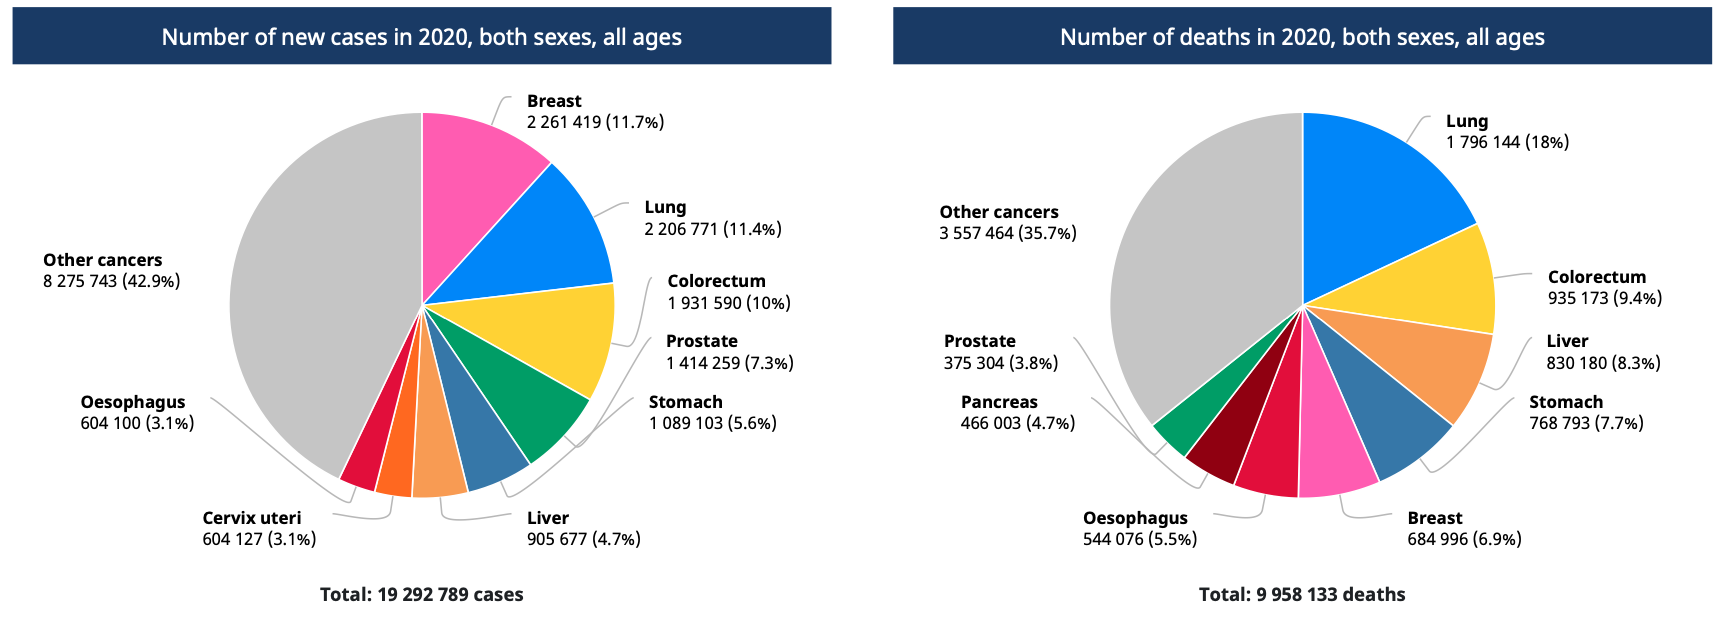
\includegraphics[width=\linewidth]{../images/cancerstats.png}
	\caption{World's cancer cases and deaths. From \cite{cancerstats} }
\end{figure}
\\
Screening and diagnosis methods for colorectal cancer can be based on different techniques. 
The gold standard in medical routines is colonoscopy which is an invasive technique\cite{jovana}.
Among medical imaging techniques, Magnetic Resonance Imaging (MRI) and Computed Tomography (CT) are the most used\cite{tesicoppola}. 
In particular Magnetic Resonance Imaging (MRI) is used for pre-operative predictions and for the evaluation of the neo-adjuvant therapy of patients affected by colorectal cancer \cite{tesicoppola}.

\begin{figure}[htp]

    \centering
    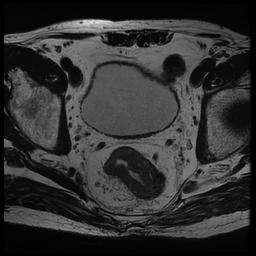
\includegraphics[width=.3\textwidth]{../images/T2AX_Alta_8.png}\hfill
    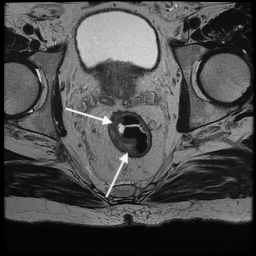
\includegraphics[width=.3\textwidth]{../images/T2AX_BO11_5.png}\hfill
    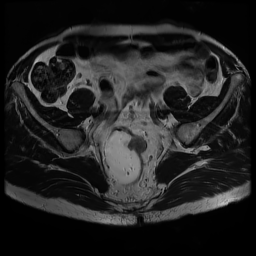
\includegraphics[width=.3\textwidth]{../images/T2AX_BO1_9.png}
    
    \caption{Example of MRI scans of patients affected by colorectal cancer. From Sant'Orsola original Dataset.}
    \label{trittico}
    
    \end{figure}
In order to get information about diagnosis, therapy evaluation, stage of colorectal cancer, analysis on radiological images can be performed through the application of dedicated algorithms.\\
In this scenario, the correct and fast identification of the cancer regions is a fundamental task. 
Up to now, this segmentation task is performed using manual or semi-automatic techniques, which are time-consuming (requiring hours per day) and subjected to the operator expertise since it requires the interaction with trained specialists\cite{tesicoppola, jovana}.
Moreover, due to the highly sensitivity to the operator expertise, the  obtained results cannot be reproduced\cite{Trebeschi2017}.
To overcome these issues, an automatic and fast way is required.\\
The aim of this project is to provide an automated pipeline to predict the response to neo-adjuvant chemo-radiotherapy of patients affect by colorectal cancer. 
The work is based and tested on MRI scans provided by IRCCS Sant’Orsola-Malpighi Policlinic.\\
The discussion will start focusing on medical digital images to understand their properties and features.
After that, an overview on the main segmentation method for the identification of the cancer regions will be given.
Then, the main pipeline characteristics and structure will be described.
In particular, how the segmentation was achieved using a Convolutional Neural Network and how extracting and processing medical image features.
Finally, the result will be shown and discussed.





\end{document}
\documentclass{standalone}
\begin{document}

    % MATERIALS AND METHODS
    \documentclass{standalone}
\begin{document}
\chapter{Results}
This Chapter will be aimed to show and discuss the results of the developed pipeline.
First of all, a brief description of the Dataset provided by the IRCCS Sant’Orsola-Malpighi Policlinic will be provided.
Then, the accuracy of the segmentation and of the prediction of response.
Finally, the outputs of the implementation will be shown.

\end{document}

    % MEDICAL DIGITAL IMAGES
    \documentclass{standalone}
\begin{document}
\section{Medical Digital Images}

A medical digital image is the digital representation of the anatomical (or functional) structure of the patient.
It is composed by a finite number of elements called \textit{pixels}.
A pixel is a discrete numeric representation of intensity or gray-level. It is an output coming from a two-dimensional function $f(x, y)$. 
The input of this function consists in the spatial coordinates, denoted with $(x, y)$ on the x-axis and y-axis of the image plane\cite{Gonzalez}.\\
A digital image can be processed by computers.
This process is called \textit{digital image processing} and it can be divided into two main categories: (\textit{image processing}) and (\textit{image analysis}).
The former includes methods whose output and input data are images.
The latter includes methods whose input data can be images and the output data are attributes extracted from the images.
\end{document}


        % GENERAL PROPERTIES 
        \documentclass{standalone}
\begin{document}
\subsection{General Properties}
The physical meaning of the image data depends on the performed image modality.
For example, Computed Tomography (CT) and Magnetic Resonance Imaging (MRI), give structural information about the anatomy of the patient.
Other techniques, such as Positron Emission Tomography (PET) or Functional Magnetic Resonance Imaging (fMRI) give information about the functional properties of the patient's target organs. 
However, we can distinguish some general characteristics of digital images:

\paragraph{Pixel depth} is the number of bits used to encode the values of each pixel and it is related to the memory space used to store the amount of the encoded information\cite{Larobina}. 
Higher the number of bits, higher the information stored but more memory space is required\cite{Larobina}. 
A group of 8 bits is called \textit{byte} and represent the smallest quantity that can be stored in the memory of a computer.
For example, if an image has a pixel depth of 16 or 12 bits the computer will always store two bytes per pixel\cite{Larobina}.
With a pixel depth of 8 bits it is possible to codify and store integer numbers between 0 and 255 $(2^8-1)$.
There are also two formats for the encoding in binary of floating-point numbers: single precision 32-bit and double precision 64-bit.

\paragraph{Pixel data} represent numerical values of the pixels stored according to the data type.
Pixel data can be complex values even if this data type is not common and can be bypassed by storing the real and imaginary parts as separate images.
For example, complex data are provided in MRI acquired data before the reconstruction (the so called k-space)\cite{Larobina}.


\paragraph{Metadata} are information that describe the image. It is usually stored at the beginning of the file as a header\cite{Larobina}. 
In the case of medical images, metadata have an important role due to the nature of the images.
For example, a magnetic resonance image might have parameters related to the pulse sequence used, timing information, number of acquisitions while a PET image might have information about the radiopharmaceutical injected and the weight of the patient.


\end{document}

        % MEDICAL IMAGE FORMATS
        \documentclass{standalone}
\begin{document}
    
\subsubsection{DICOM Format}

Image file formats provide a standard way to store information of an image in a computer file\cite{biondi}.
DICOM is the acronym of Digital Imaging and COmmunications in medicine.
It is not only a file format but also a network communication protocol\cite{Larobina}.
However here, we will discuss DICOM only as a medical image format.\\
DICOM file format establishes that the pixel data cannot be separated from the metadata\cite{Larobina}.
In other words, metadata and pixel data are merged in a unique file.
The header contains the description of the entire procedure used to generate the image in terms of acquisition protocol and scanning parameters\cite{Larobina}. 
It also contains patient information such as name, gender, age. 
For these reasons, the DICOM header is modality-dependent and varies in size. 
In practice, the header allows the image to be \textit{self-descriptive}.

\end{document}

        % SPATIAL DOMAIN FILTERING
        \documentclass{standalone}
\begin{document}
\section{Spatial Domain Filtering}


Filtering is a procedure used for modifying or enhancing an image.
The value of any given pixel in the output image is determined by applying some operations to the neighborhood of the corresponding input pixel.
A pixel's neighborhood is some set of pixels, defined by their locations relative to that pixel.
The term \textit{spatial domain} indicates that the procedures operate directly on pixels.
Mathematically:

\begin{equation}
    g(x,y) = T[f(x,y)] 
\end{equation}

where $f(x, y)$ is the input image, $g(x, y)$ the output image and $T$ is an operator on $f$ defined over some neighborhood of $(x, y)$.
The operation on the point located in $(x, y)$ usually involves the application of a matrix called \textit{mask} or \textit{kernel}.
The application of the above-mentioned mask (or kernel) on an image is called \textit{spatial filtering}.
Filtering creates a new pixel with the same coordinates of the center of the neighborhood, whose value is the result of the operation.
For each $(x, y)$ of the image, the filter transform $g(x, y)$ is the linear combination of the mask coefficient $w(s, t)$ and the pixels of the image affected by the mask itself.
In general, we can write:
\begin{equation}
    g(x, y) = \sum_{s = -a}^{a} \sum_{t = -b}^{b} w(s, t) f(x + s, y + t)
\end{equation}  

\begin{figure}[ht]

    \centering
    \includegraphics[width=.9\textwidth]{../images/filtering.png}
    
    \caption{Example of spatial filtering. A filtered image is generated as the center of the mask or kernel, moves to every pixel in the input image. From \cite{filtering}}
    \label{filtering}
\end{figure}


\end{document}

        % SMOOTHING FILTERS
        \documentclass{standalone}
\begin{document}
\subsection{Smoothing Filters}
Smoothing filters are used for blurring and for noise reduction\cite{corrandconv}.
This is used in removal of small details and bridging of small gaps in lines or curves.
Smoothing spatial filters include \textit{linear filters} and \textit{nonlinear filters}\cite{corrandconv}.\\
The general implementation for filtering an $M \times N$ image with a weighted averaging filter of size $m \times n$ is given by:
\begin{equation}
    g(x, y) = \frac{\sum_{s = -a}^{a} \sum_{t = -b}^{b} w(s, t) f(x + s, y + t)}{\sum_{s = -a}^{a} \sum_{t = -b}^{b} w(s, t)}
\end{equation}
where $m=2a+1$ and $n=2b+1$.

\paragraph{Linear filtering} is based on the \textit{mean filter} \cite{filters}.
The mean filter is a simple sliding spatial filter that replaces the center value in the mask region with the average of all the neighboring pixel values including itself. 
These filters are also called \textit{low pass filters} since the process of averaging drastically lowers high frequencies.
The mask or kernel is a square.
Larger kernels ($5\times5$ or $7\times7$) produce more denoising that smaller ones ($3 \times 3$) but make the image more blurred\cite{filters}. 
A common mean filter can be described by a $3\times3$ matrix with all elements equal to 1, so that the output pixel corresponds to a value of:

\begin{equation}
    R = \frac{1}{9} \begin{pmatrix}
        1 & 1 & 1\\
        1 & 1 & 1\\
        1 & 1 & 1
        \end{pmatrix} \mathbf{z} = \frac{1}{9} \sum_{i = 1}^{9}z_i
\end{equation}

 or using a weighted mean filter:

\begin{equation}
     R' = \frac{1}{16}\begin{pmatrix}
        1 & 2 & 1\\
        2 & 4 & 2\\
        1 & 2 & 1
        \end{pmatrix} \mathbf{z}
\end{equation}






\paragraph{Non-Linear filtering} is based on the \textit{median filter}\cite{filters}.
The median filter principle is similar to the mean filter. 
The mask or kernel is scanned over the pixels of the entire image.
The median of the pixel values in the mask region is calculated, and the center pixel of the mask region is replaced with the calculated median value\cite{filters}.
This filter is particularly effective in the presence of \textit{impulse noise} (or \textit{salt-and-pepper noise})\cite{corrandconv}.\\
Mathematically:

\begin{equation}
    g(p) = median\{f(p), where \: p \in N_8(p)\}
\end{equation}
where $g(p)$ is the median pixel value, $f(p)$ all pixel values under mask, and $N_8(p)$ 8-neighborhood of pixel $p$.


\paragraph{\textcolor{blue}{Notes:} Adaptive filters} 
are commonly used in image processing to enhance or restore data by removing noise without significantly blurring the structures in the image\cite{Adaptive}.
This means not smoothing the areas of the image in which there is a large jump in intensity values (i.e. when there is an \textit{edge}) and at the same time applying the filter to lower the noise.
In this case, the local variance will be evaluated concerning the variance of the noise that occurs.\\
Mathematically:
\begin{equation}
    \hat{f}(x, y) = f(x, y) - \frac{\sigma_{noise}^2}{\sigma_{local}^2}[f(x, y) - m_{local}]
\end{equation}

\end{document}

    % SEGMENTATION
    \documentclass{standalone}
\usepackage{xr}
\externaldocument{../Chapter2/intro}
\begin{document}
\subsection{Segmentation}
Once trained, the CNN model was used for the segmentation of the MRI scans of each patient.
Before the segmentation, the scans are pre-processed as previously described.
\\
The segmentation is done slice by slice, for each patient, by using the trained CNN model to obtain the predicted tumor area.
The prediction values range between 0 and 1.
\\
Then, using \textsc{OpenCV}\cite{opencv_library} functions it is possible to obtain a segmented area like the one in Figure \ref{contoured}, where the red contour represents the border of the predicted tumor area.


\begin{figure}[htp]

    \centering
    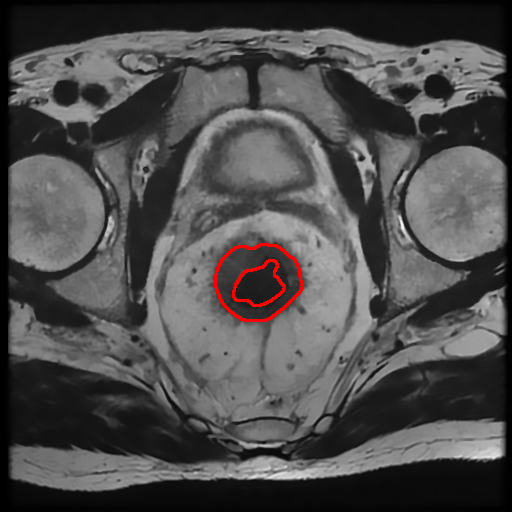
\includegraphics[width=.49\textwidth]{../images/BO56_9_cont.png}
    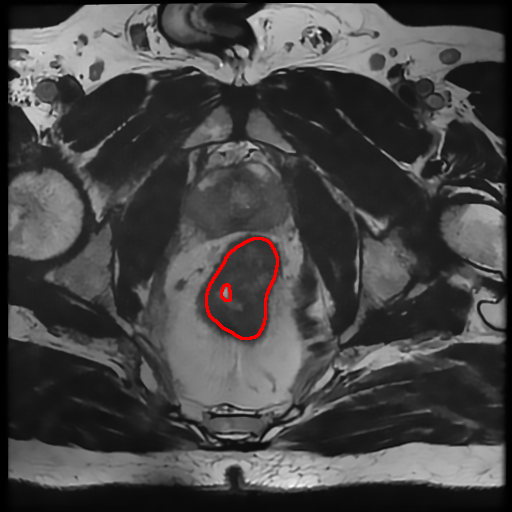
\includegraphics[width=.49\textwidth]{../images/BO85_6_cont.png}
    
    \caption{Images of colorectal cancer with identified tumor areas from two different patients. The red contour represents the border of the predicted tumor area.}
    \label{contoured}
    
    \end{figure}


\end{document}

        % METHODS
        \documentclass{standalone}
\begin{document}
\subsection{Methods}
During the year several segmentation methods have been developed\cite{biondi}.
There are several ways to classify these methods.
For example, depending if they require or not a training set of data, they can be classified into \textit{supervised} or \textit{unsupervised} methods.
More, they can be classified depending on the information type they use, like \textit{Pixel classification} methods, which use only information about pixel intensity, or \textit{Boundary following} methods which use edge information etc...\cite{biondi}.\\
Among the most common ones:

\paragraph{Thresholding}
is a very simple and common approach to segmentation.
This method is applied on the \textit{histogram} of the image.
The histogram of a digital image with intensity levels $L$ in the range $[0, \: L-1]$, is a discrete function $h(l_k) = n_k$ where $l_k$ is the k-th intensity value and $n_k$  is the number of pixels with intensity $l_k$.\\
Thresholding consists in binarizing an image through an (if) clause on the intensity value of each point after having determined a threshold value $T \in [0, \: L-1]$.
The threshold value $T$ is usually chosen by visual assessment on the image histogram but it can be automatize by algorithms like the \textit{Otsu algorithm}.
One drawback of this method is that some parts of the image can belong to the same class even if they belong to different objects.
In fact, thresholding does not take into account the spatial characteristics of the image.
Moreover, it is sensitive to noise and intensity inhomogeneity that corrupt the image histogram and make difficult the classification of pixels\cite{biondi}.

\begin{figure}[htp]

    \centering
    \includegraphics[width=.45\textwidth]{../images/thresholdhistogram.png}
    \includegraphics[width=.45\textwidth]{../images/thresholdexample.png}
    
    \caption{Example of thresholding segmentation using Fiji software\cite{Fiji}. \\
    \textit{ Left)} Image Histogram.\textit{ Right)} Result of thresholding.}
    \label{thresholding}
    
    \end{figure}


\paragraph{Artificial Neural Networks} 
are computational architectures derived from neural physiological models\cite{segmentationreview}.
Artificial Neural Networks (ANNs) have evolved into a broad family of techniques.
For visual analysis are usually used Convolutional Neural Networks (CNNs) based on \textit{convolution kernels} or \textit{filters} that slide along input data to extract feature maps\cite{wiki:cnn}.
Several architectures have been developed over the years, for different tasks and fields of application.
In bio-medical image processing, the so-called U-Net\cite{unet}, is one of the most common architecture.
U-Net is a kind of CNN which allows overcoming the requirement of many training data\cite{biondi, unet}.
However a better explanation of ANNs will be provided in the following chapter.




\end{document}
        
        % UNET
        \documentclass{standalone}
\begin{document}
\section{U-Net}
The U-net is a convolutional network architecture for fast and precise segmentation of images especially in the biomedical field\cite{unet}.
One of the main advantage of the U-net is the ability of dealing with small dataset. The name U-net refers to the U shape of the network architecture. 
The whole structure is divided into two main parts, as shown in Figure\ref{fig:unet}:

\paragraph{Encoder}:
or contraction path is a sequence of convolutional and max pooling layers with the aim of extracting features and reducing dimensionality.

\paragraph{Decoder}:
or expansion path is a sequence of transpose convolutional layers to with the aim of reconstruct the feature map and consequently the segmentation mask.
\begin{figure}[htp]

    \centering
    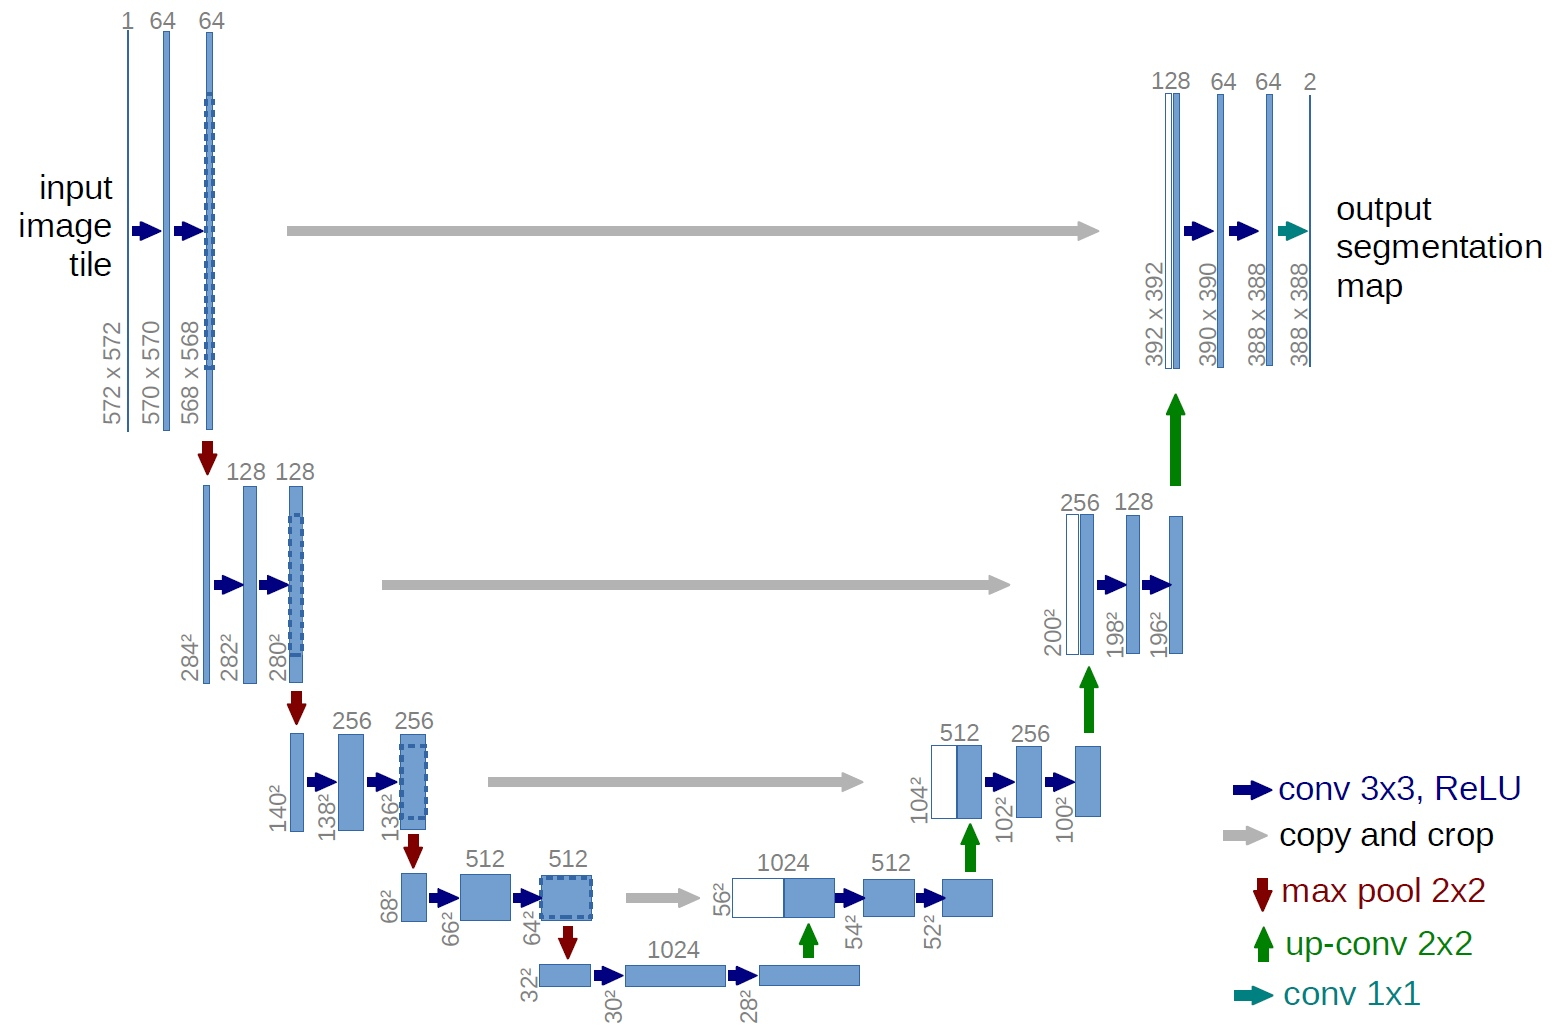
\includegraphics[width=.9\textwidth]{../images/U-Net arch.jpeg}
    
    \caption{Original U-Net architecture. From\cite{unet}}
    \label{fig:unet}
    
    \end{figure}
\\
The \textit{Encoder} is a typical Convolutional Neural Network that consists in the repeated application of convolutions, followed by ReLu activation function and max pooling operations.
During the contraction the input size is decreased and so the spatial information, while the information about features is increased.
The \textit{Decoder} combines the features extracted in the contraction path  with tha spatial information by a sequence of transpose convolutions (or up-convolutions) and concatenations (grey arrows in Figure\ref{fig:unet}).



\end{document}
    
    % RADIOMICS
    \documentclass{standalone}
\begin{document}
\section{Radiomics}
Radiomics consists in methods that extract from medical images a large number of features, which have the potential to uncover disease characteristics that fail to be appreciated by the naked eye\cite{wiki:Radiomics}.
The main objective of radiomics is to assist the subjective interpretation of the clinicians with an objective prediction.
In the new era of precision medicine, radiomics is an emerging translational research field that aims to find associations between qualitative and quantitative information extracted from clinical images and clinical data to support the decision making process\cite{tesicoppola}.
Radiomic features can be divided into different classes:
\begin{itemize}
    \item First Order Statistics
    \item Shape based features 2D and 3D
    \item Gray Level Co-occurrence Matrix (GLCM)
    \item Gray Level Size Zone (GLSZM)
    \item Gray Level Run Length Matrix (GLRLM)
    \item Neighbouring Gray Tone Difference Matrix (NGTDM)
    \item Gray Level Dependence Matrix (GLDM)
\end{itemize}

\end{document}

        % POSSIBLE PURPOSES OF RADIOMICS
        \documentclass{standalone}
\begin{document}
\subsection{Possible Purposes Of Radiomics}

The possible applications of radiomics are based on a very wide range, from the prediction of clinical outcomes to the oncological diagnosis.
In this subsection, a brief overview of some general possible purposes will be given.
\subsubsection{Prediction of clinical outcomes} 
Radiomic features may be useful for predicting patient survival and describing intratumoral heterogeneity as demonstrated in a study by Aerts et al. \cite{Aerts}.
More, the usefulness of radiomics for predicting the immunotherapy response of patients with non-small cell lung cancer (NSCLC) using pretreatment CT and PET-CT images has been demonstrated by other studies\cite{tesicoppola}.
\subsubsection{Prediction of metastases}
Radiomic features can also predict the metastatic stage of tumors. 
For example, many radiomic features were identified as predictors of distant metastasis of lung adenocarcinoma in a study by Coroller et al.\cite{Coroller}.
They concluded that radiomic features may be useful in identifying patients at high risk of developing distant metastases, guiding clinicians in choosing the most effective treatment for individual patients.
\subsubsection{Prediction of physiological events}
Another possible application of radiomics analysis is the prediction of physiological events. 
Indeed, radiomics can be applied for the characterization and investigation of complex physiological events such as brain activity, which is usually studied with specific imaging techniques such as functional magnetic resonance ”fMRI”\cite{tesicoppola}. 


\end{document}
    \newpage
    % PCA
    \documentclass{standalone}
\begin{document}
\markboth{CHAPTER 1. MATERIALS AND METHODS}{1.5. PCA}
\section{Principal Component Analysis}
Principal component analysis (PCA) is a technique to reduce data dimensionality.
It replaces the $n$ original variables by a smaller number, $q$, of linear combinations, called principal components, of the original variables.
The application areas include data compression, image analysis, pattern recognition, regression and classification prediction\cite{PCA}.\\
The most common definition of PCA, due to Hotelling, states that for a set of observed data vectors 
$ \{ \mathbf{t}_{n} \}$, $n \in \{1, \dots, N \} $, the $q$ principal axes $\mathbf{w}_j$, $j \in \{ 1, \dots, q \} $ are those orthonormal axes onto which the retained variance under projection is maximal.
The vectors $\mathbf{w}_j$ are given by the $q$ dominant eigenvectors (i.e. those with the largest associated eigenvalues $\lambda$) of the sample covariance matrix $\mathbf{S} = \sum_{n}^{} ( \mathbf{t_n} - \mathbf{\bar{t}}) ( \mathbf{t_n} - \mathbf{\bar{t}})^T / N$ such that  $ \mathbf{S}\mathbf{w}_j = \lambda_j \mathbf{w_j}$ and where $\mathbf{\bar{t}}$ is the sample mean.
The vector $\mathbf{x}_{n} = \mathbf{W^T} (\mathbf{t_n} - \mathbf{\bar{t}})$, where $ \mathbf{W} = (\mathbf{w}_1 , \mathbf{w}_2 \dots \mathbf{w}_j)$ is thus a q-dimensional reduced representation of the observed vector $\mathbf{t}_{n}$ \cite{PCA}.
As we have mentioned, $\lambda_j$ is just the variance of each new feature dimension.
How to choose an appropriate $q$ depends on the Variance Contribution Rate  $\alpha_j = \lambda_j / \sum_{j}^{} \lambda_j $. 
This can be determined by looking at the cumulative explained variance ratio as a function of the number of components as shown in figure \ref{cumulativevr}.


\begin{figure}[ht]

    \centering
    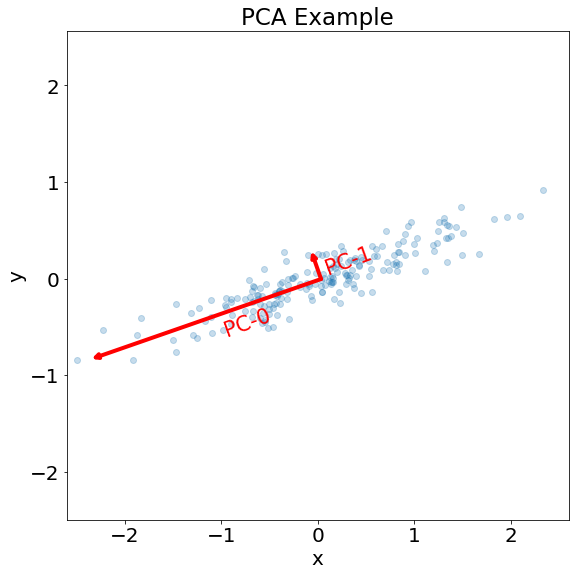
\includegraphics[width=0.62\textwidth]{../images/PCAexample1.png}
    
    \caption{Example of Principal Component Analysis.
     The red vectors represent the principal axes of the data, and the length of the vector is an indication of the variance of the data when projected onto that axis.}
    \label{PCAexample}
    
    \end{figure}

\markboth{CHAPTER 1. MATERIALS AND METHODS}{1.5. PCA}

\begin{figure}[htp]

    \centering
    \includegraphics[width=.68\textwidth]{../images/cumulative3.png}
    
    \caption{Example of cumulative explained variance ratio as a function of the number of components. This curve quantifies how much of the total variance is contained within the first N components. We can see that the first 10 components contain approximately $75 \%$ of the total variance, while to the reach the $100 \%$ you need around 50 components.}
    \label{cumulativevr}
    
    \end{figure}

\end{document}

    % SVM
    \documentclass{standalone}
\begin{document}
\markboth{CHAPTER 1. MATERIALS AND METHODS}{1.6. SVCs}
\section{Support Vector Classifiers}

Support Vector Classifiers (SVCs) are a subclass of Support Vector Machines (SVMs) that are a set of supervised learning methods (i.e. requires training data) used for purposes such as classification and regression.
A Support Vector Machine constructs a hyper-plane or set of hyper-planes in a high or infinite dimensional space.
Intuitively, a good separation is achieved by the hyper-plane that has the largest distance to the nearest training data points of any class (functional margin), since in general the larger the margin the lower the generalization error of the classifier\cite{SVCscikit, Bishop}.\\
For a SVC, mathematically, given training vectors $ \mathbf{x}_i \in \mathbb{R}^p ,  \: i \in \{1,\dots, n\} \:$, in two classes, and a vector $\mathbf{y} \in \{ -1, \: 1 \}^n$ (or $ \{0, \: 1 \}^n$), the goal is to find $\mathbf{w} \in \mathbb{R}^p$ and $b \in \mathbb{R}$ such that the prediction given by $sign(\mathbf{w^T  \mathbf{\Phi(x)}} + b)$ is correct for most samples \cite{SVCscikit}.\\
The function $\Phi(x)$ provides a convenient way of extending the analysis from the input space to a non-linear feature space by using a high-dimensional mapping. 
Finding a linear separating hyperplane in this feature space is equivalent to finding a non linear decision boundary in the input space\cite{SVCmapping}.\\
A SVC solves a primal problem and a dual problem. 
The primal:
\begin{equation}
    \min_{w, \zeta} \frac{1}{2} (\mathbf{w}^T  \mathbf{w}) + C \sum_{i = 1}^{n} \zeta_i
\end{equation}

subject to: $\begin{cases}
    y_i \cdot (\mathbf{w}^T  \mathbf{\Phi(x_i)} + b)  \geq 1 - \zeta_i, \\
    \zeta_i \geq 0 \quad i = 1, \dots, n 
    \end{cases}$
\newline
\\
\\
From an intuitive point of view, the minimization ($\mathbf{w}^T  \mathbf{w}$) corresponds to maximize the functional margin while incurring a penalty when a sample is misclassified or within the margin boundary.
The penalty term C controls the strength of this penalty, and acts as an inverse regularization parameter\cite{SVCscikit}.
Ideally, the term $\zeta_i$ should be 0 for a perfect prediction but real data are usually not always perfectly separable with a hyperplane, so some samples will be at a distance $\zeta_i$ from their correct margin boundary.
\\
The dual problem instead:
\begin{equation}
    \min_{\alpha} \frac{1}{2} (\mathbf{a}^T \mathbf{Q} \mathbf{a}) - \mathbf{e}^T \mathbf{a}
\end{equation}

subject to: $\begin{cases}
    \mathbf{y}^T \mathbf{a} = 0, &  \\
    0 \leq a_i \leq C  &  i = 1, \dots, n
    \end{cases}$
\newline
where $\mathbf{e}$ is the vector of all ones, $\mathbf{Q}$ is a $n \times n$ matrix: $Q_{ij}\equiv y_i y_j K(\mathbf{x_i}, \mathbf{x_j})$ where $K(\mathbf{x_i}, \mathbf{x_j}) = \mathbf{\Phi(x_i)}^T \mathbf{\Phi(x_j)} $ is the so called \textit{kernel}.
The $a_i$ terms are called \textit{dual coefficients}, and they are upper-bounded by C.\\


\newpage
\markboth{CHAPTER 1. MATERIALS AND METHODS}{1.6. SVCs}
Once these problems are solved, for a sample $\mathbf{z}$, the decision function is given by: 
\begin{equation}
    \sum_{i \in SV}^{}  y_i a_i \mathbf{K(x_i, z)} + b
\end{equation}
where the sum is over the supported  vectors (SV) that are the samples that lie within the margin because the dual coefficients $a_i$ are zero for the other samples\cite{SVCscikit}.

\begin{figure}[ht]

    \centering
    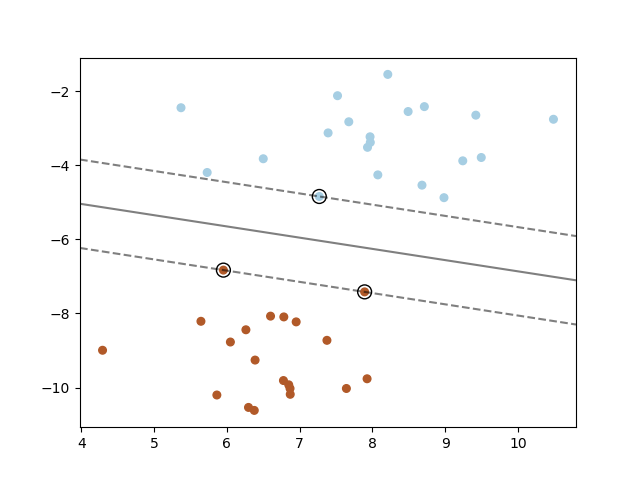
\includegraphics[width=.95\textwidth]{../images/svcexample.png}
    
    \caption{Classification made by a Support Vector Classifier (SVC) for a linearly separable problem. The gray line represents the line of the separation hyper-plane. The three samples on the margin boundaries (dashed lines) are called \textit{support vectors}. From \cite{SVCscikit}}\label{fig:svc}
    
    
    \end{figure}

\end{document}


\end{document}
\documentclass{standalone}
\begin{document}

    % INTRO
    \documentclass{standalone}
\begin{document}
\chapter{Results}
This Chapter will be aimed to show and discuss the results of the developed pipeline.
First of all, a brief description of the Dataset provided by the IRCCS Sant’Orsola-Malpighi Policlinic will be provided.
Then, the accuracy of the segmentation and of the prediction of response.
Finally, the outputs of the implementation will be shown.

\end{document}
\newpage
        % PIPELINE WORKFLOW
        \documentclass{standalone}
\begin{document}
\section{Pipeline Workflow}

As we have seen, the pipeline workflow is divided into many steps, each one performing a different task. 
In this section, I will describe in details how each step of the pipeline is achieved. 
This section involves only a description. 
The implementation will be discussed in the next one.

\end{document}

            % PRE-PROCESSING
            \documentclass{standalone}
\begin{document}
\subsection{Pre-processing}

This preliminary step is performed before the training and segmentation process.
It involves the application of the non-local means algorithm to remove possible noise sources and a gamma correction to improve the image contrast.\\
First of all, the MRI scans are acquired from the dataset, slice by slice, in DICOM format and converted into pixel arrays with the original pixel depth in order to preserve all the original information.
Then, to have pixel data in the range $ [ 0, \: 1 ] $, images are normalized and rescaled to binary floating point 32-bit.
This is required to work with \textsc{TensorFlow}\cite{Tensorflow} and \textsc{Keras'} \cite{Keras} functions that deal with the segmentation process, as you will see in the implementation section.
\\
The images are then filtered by using the non-local means algorithm.
In Figure \ref{noisydenoised}, you can see the an example of application of the non-local means algorithm on the same MR image of a patient affected by colorectal cancer.
The original image on the \textit{left}, is affected by noise while the filtered one, on the \textit{right}, results smoothed without significant detail loss. 
In fact, one drawback of smoothing filters is the blurring of small details but in this case, they are preserved.
This behavior is reflected in the image histogram. 
As you can see in Figure \ref{histo}, the original image histogram (red) is affected by great fluctuations of pixel intensity, that highlight the presence of noise. 
Instead, the denoised image histogram (blue) results in a smoothed histogram, preserving the original shape.
\\
After performing the non-local means algorithm, the image contrast is enhanced by a gamma correction.
In this case, the $\gamma$ parameter has been set to a value of 1/1.5 to make darker regions lighter.
An example of the performed gamma correction can be seen in Figure \ref{denoisedgamma}.
Moreover, the rise of contrast can be noticed on the gamma-corrected image histogram, shown in Figure \ref{histogamma}.
\\
In summary, the preprocessing steps are:
\begin{itemize}
    \item normalization and rescaling
    \item denoising
    \item gamma correction
\end{itemize}

A comparison of the image before and after the pre-processing can be seen in Figure \ref{noisyfinal}.

\begin{figure}[htp]

    \centering
    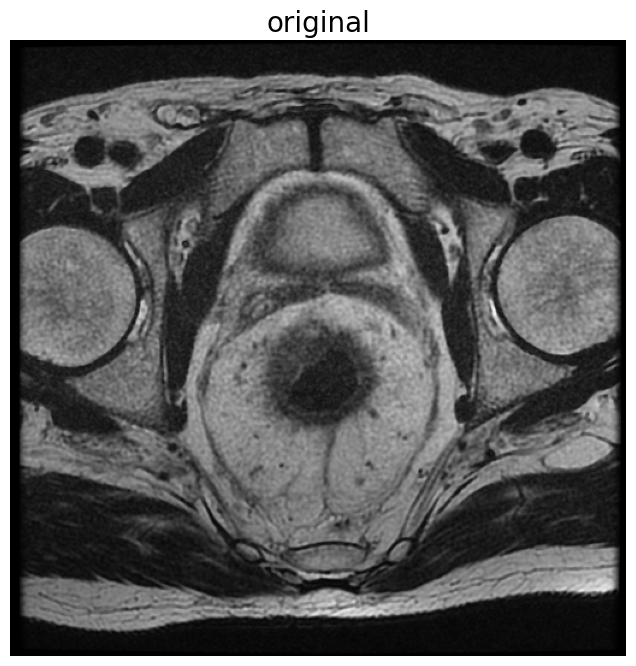
\includegraphics[width=.49\textwidth]{../images/noisy.png}
    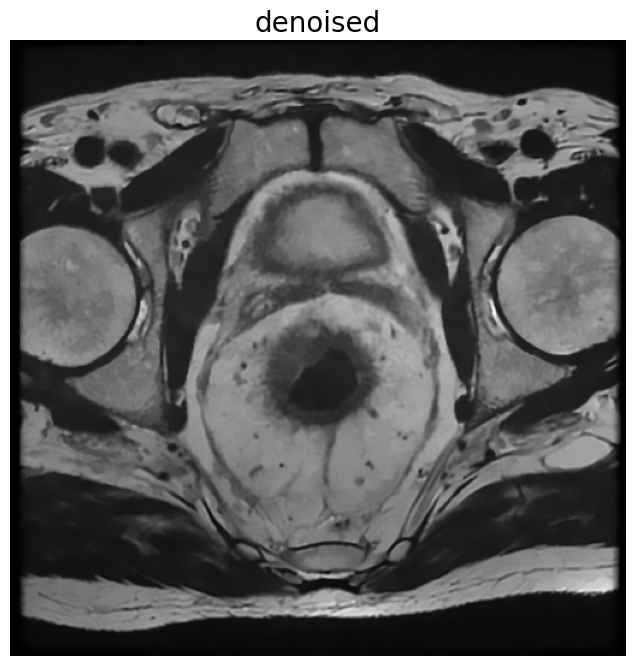
\includegraphics[width=.49\textwidth]{../images/denoised.png}
    
    \caption{ \textit{ Left)} Original MR image of a patient affected by colorectal cancer.\textit{ Right)} The same image after non-local mean algorithm.}
    \label{noisydenoised}
    
    \end{figure}

\begin{figure}[htp]

    \centering
    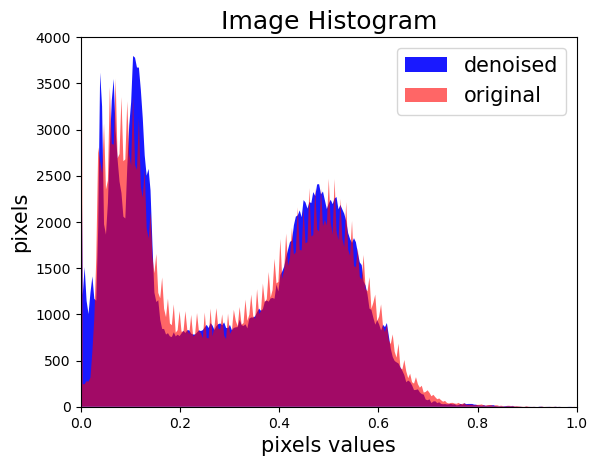
\includegraphics[width=0.73\textwidth]{../images/histogram.png}

    
    \caption{Original vs denoised image histogram. The original image histogram (red) is affected by great fluctuations of pixel intensity, highlighting the presence of noise. The denoised one (blue) results in a smoothed histogram, preserving the original shape.}
    \label{histo}
    
    \end{figure}

\begin{figure}[htp]

    \centering
    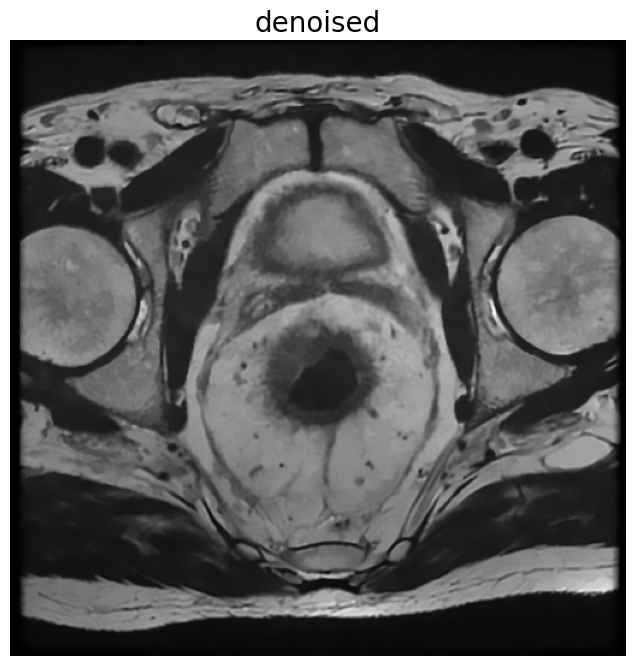
\includegraphics[width=.49\textwidth]{../images/denoised.png}
    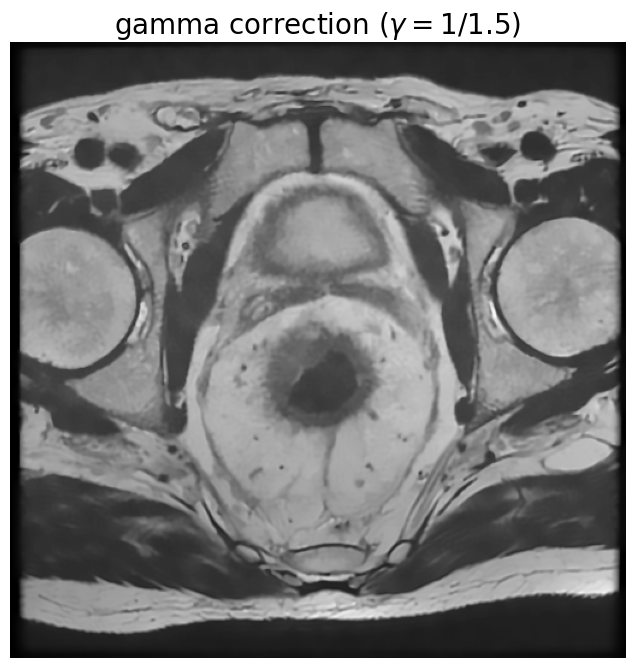
\includegraphics[width=.49\textwidth]{../images/gammacorrection.png}
    
    \caption{ \textit{ Left)} denoised MR image of a patient affected by colorectal cancer.\textit{ Right)} The same image after gamma correction.}
    \label{denoisedgamma}
    
    \end{figure}

\begin{figure}[htp]

    \centering
    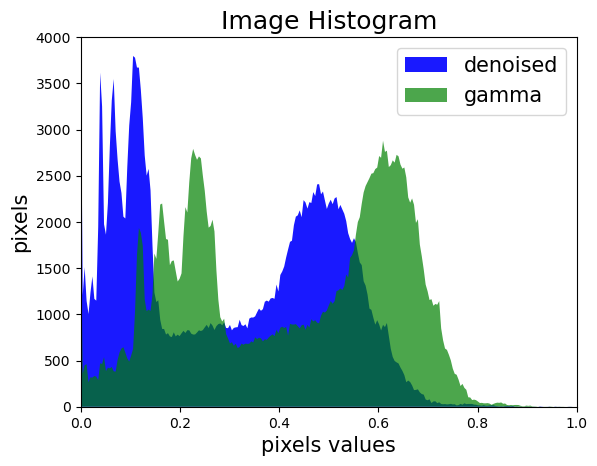
\includegraphics[width=0.73\textwidth]{../images/gammahist.png}

    
    \caption{Denoised vs gamma-corrected image histogram. The gamma-corrected image histogram (green) results in a right-shifted histogram.}
    \label{histogamma}
    
    \end{figure}

\begin{figure}[htp]

    \centering
    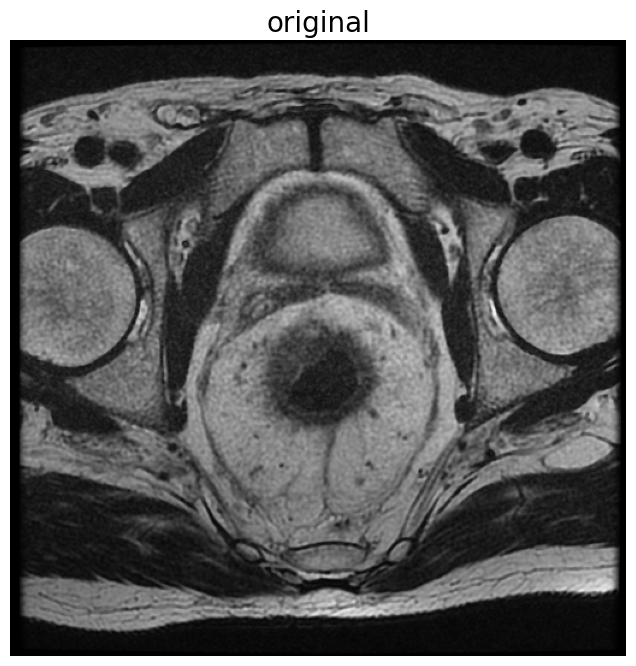
\includegraphics[width=.49\textwidth]{../images/noisy.png}
    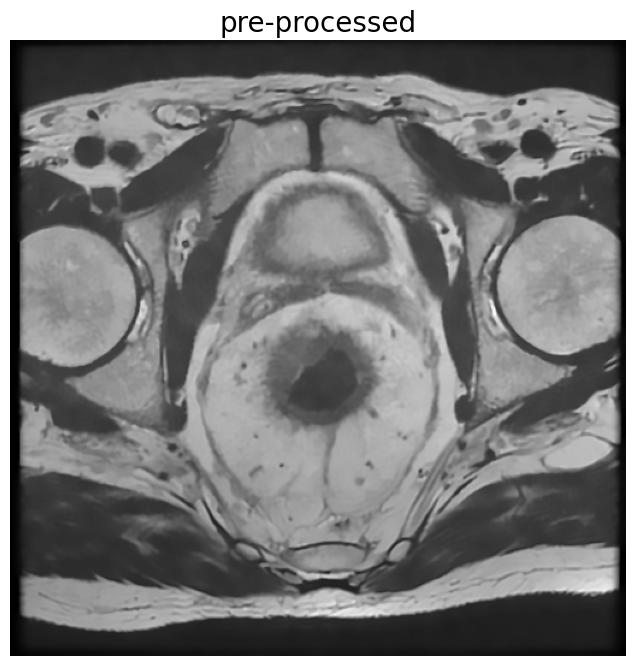
\includegraphics[width=.49\textwidth]{../images/finalimage.png}
    
    \caption{ \textit{ Left)} Original MR image of a patient affected by colorectal cancer.\textit{ Right)} The same image after the pre-processing steps.}
    \label{noisyfinal}
    
    \end{figure}
\end{document}
\newpage
            % CNN-TRAINING
            \documentclass{standalone}
\usepackage{xr}
\externaldocument{../Chapter1/Section3/Subsection3/Unet}
\begin{document}
\subsection{Training}

This step is one of the most important since the Convolutional Neural Network (CNN) model coming from the training process will be used for the segmentation of the images.
\\
Before proceeding with the training, the MRI scans and the medical annotation of each patient were manually checked since for some of them there was misregistration between the image and the medical annotation (i.e. the medical annotation did not correspond to the correct slice).
The medical annotations consist of a set of $(x, y)$ points that border the tumor area on the image.
Pixels inside the bordered area were labeled with a value of 255 while the other ones with 0.
\\
The images were then selected and stored in the proper directories, one for the images in DICOM format and one for the ground-truth images stored as 8-bit unsigned integers images.
\\
The training was performed by using a custom data generator which was responsible for providing the right input and ground-truth images, pre-processing them and splitting the images into training and validation sets.
\\
Some data augmentation was also performed on the training set of data, to overcome the lack of data and to reduce overfitting.
It consists in adding slightly modified copies of already existing data, using geometrical transformations such as flipping and rotations of the images.
In this particular case, the images were randomly horizontal or vertical flipped.
\\
In summary, the custom data generator provides the following steps: 
\begin{itemize}
    \item read the input images and ground-truth images from the relative directories
    \item shuffle and split data into training and validation sets
    \item pre-process the input images following the steps described in the previous subsection
    \item normalize and rescale the images
    \item zip the input images with the correct ground-truth images
    \item perform data-augmentation on training set
\end{itemize} 
An example of input and ground-truth images from the training set is shown in Figure \ref{showdataset}.
Instaed, An example of input and ground-truth images from the validation set is shown in Figure \ref{showdataset2}.
In this case no data augmentation is performed.
\\
The network architecture used for this project is a U-Net-like structure made by a contraction and expansion path.
The difference between the original architecture and the one used in this project consists of the use of a so-called \textit{backbone} which refers to the feature extracting network.
Just to clarify this notion, in Figure \ref{fig:unet}, the feature maps (blue boxes) are extracted by a series of Convolutional, ReLu, and Max-pooling layers (denoted by the arrows).
However, one can use various combinations of different layers to extract feature maps. 
So, the combination of layers can create new networks and architectures.
In this case the \textit{backbone} consists of an architecture called \textit{EfficientNetb0}\cite{EfficientNet}.
\\
The loss function is the combination between Dice loss with the binary focal loss.
\\
The algorithm used to minimize the loss function consists of the default \textit{Adam} (Adaptive Moment Estimation) optimizer provided by \textsc{TensorFlow} with a learning rate set to $0.001$.
\\
The batch size\footnote{the batch size refers to the number of samples provided in one iteration.} was set to a value of 4.
\\
The metric function used to judge the performance during the training of the model was the Dice Similarity Coefficient (DSC).

\begin{figure}[htp]

    \centering
    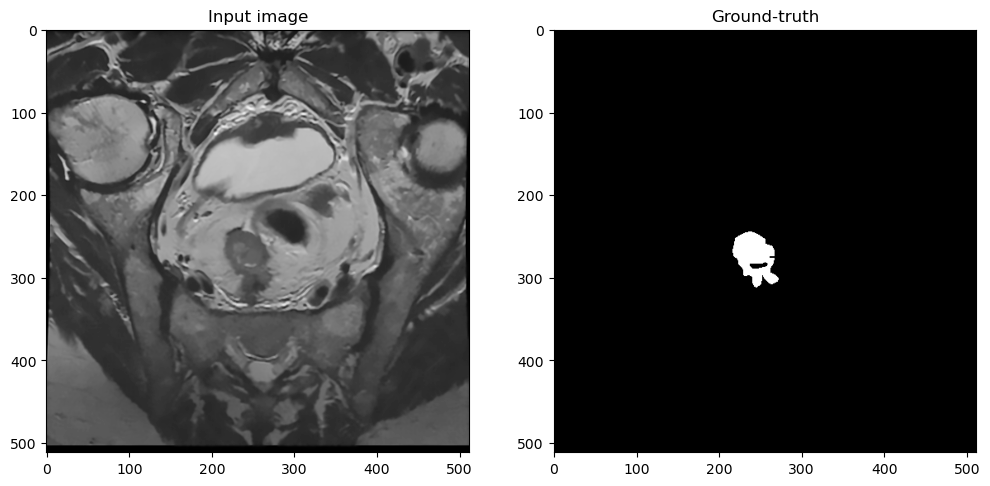
\includegraphics[width=0.9\textwidth]{../images/showdataset.png}
    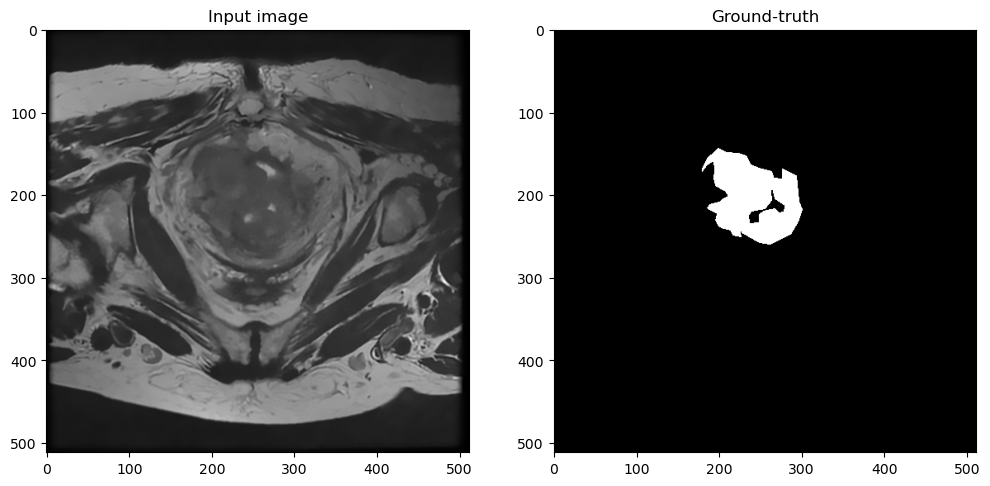
\includegraphics[width=0.9\textwidth]{../images/showdataset1.png}

    \caption{Example of input and ground-truth images from the training set.
    The white area on the ground-truth images represents the tumor area. As you can see, the images are randomly horizontally or vertically flipped. }
    \label{showdataset}
    
    \end{figure}

\begin{figure}[htp]

    \centering
    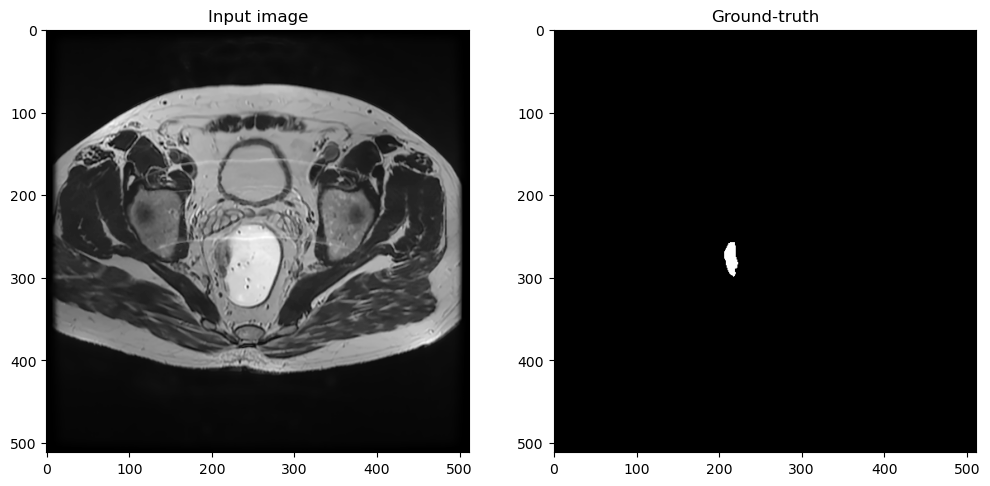
\includegraphics[width=0.9\textwidth]{../images/showdataset2.png}
    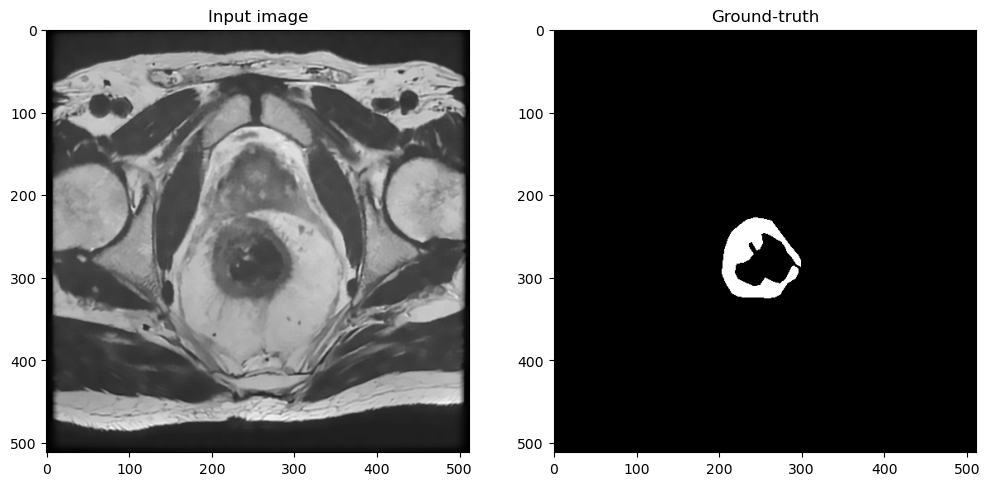
\includegraphics[width=0.9\textwidth]{../images/showdataset3.png}

    \caption{Example of input and ground-truth images from the validation set.The white area on the ground-truth images represents the tumor area. As you can see, no data augmentation was performed on this set}
    \label{showdataset2}
    
    \end{figure}

\end{document}


\newpage
            % SEGMENTATION
            \documentclass{standalone}
\usepackage{xr}
\externaldocument{../Chapter2/intro}
\begin{document}
\subsection{Segmentation}
Once trained, the CNN model was used for the segmentation of the MRI scans of each patient.
Before the segmentation, the scans are pre-processed as previously described.
\\
The segmentation is done slice by slice, for each patient, by using the trained CNN model to obtain the predicted tumor area.
The prediction values range between 0 and 1.
\\
Then, using \textsc{OpenCV}\cite{opencv_library} functions it is possible to obtain a segmented area like the one in Figure \ref{contoured}, where the red contour represents the border of the predicted tumor area.


\begin{figure}[htp]

    \centering
    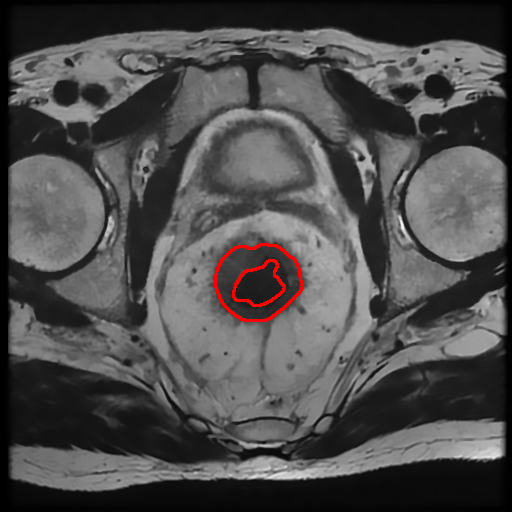
\includegraphics[width=.49\textwidth]{../images/BO56_9_cont.png}
    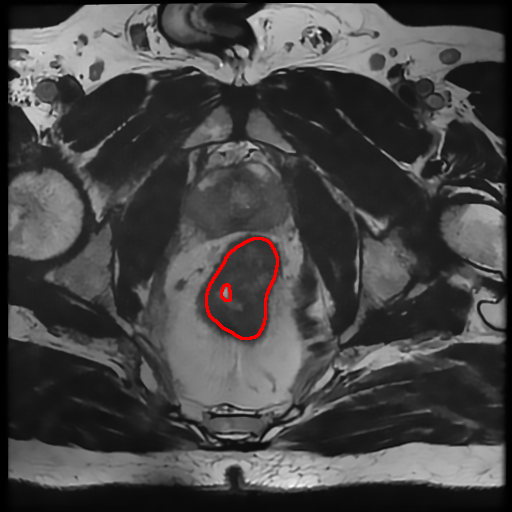
\includegraphics[width=.49\textwidth]{../images/BO85_6_cont.png}
    
    \caption{Images of colorectal cancer with identified tumor areas from two different patients. The red contour represents the border of the predicted tumor area.}
    \label{contoured}
    
    \end{figure}


\end{document}
\newpage
            % FEATURES EXTRACTION
            \documentclass{standalone}
\begin{document}
\subsection{Features Extraction}

This step consists of the extraction of the radiomic features from the images.
For this purpose, the original MRI scans of each patient and the segmented ones are saved, as 3D images in a particular format (.nrrd) required by \textsc{Pyradiomics} library \cite{Pyradiomics} to extract features from the segmented areas of every single slice of the patient. 
\\
From each patient, a total of 100 radiomic features were extracted.
The extraction settings were stored in a $\mathtt{Params.yaml}$ file required by \textsc{Pyradiomics}.
The data were then stored in a data frame containing 100 columns (one for each feature) and 48 rows (one for each patient) ready for the analysis step.


\end{document}

            % FEATURES ANALYSIS
            \documentclass{standalone}
\begin{document}
\subsection{Features Analysis}

This step came immediately after the features extraction.
Firstly, the features have been read, looking for some correlation between features since the goal is to reduce as much as possible the number of irrelevant features.
As you can see from Figure\ref{heatmap}, showing the features correlation heatmap, there is the presence of highly correlated (and anti-correlated) features, highlighted by the red (and blue) color.
The names of the features are set by \textsc{Pyradiomics}. In particular, the name before the underscore ($\_$) highlights the feature class. For example $\mathtt{glcm}$ stands for \textit{Gray Level Co-occurrence Matrix (GLCM)} or $\mathtt{firstorder}$ means that the feature belongs to that class.
\\
In order to reduce the number of features, Principal Component Analysis (PCA) was performed on the data frame containing the extracted 100 features for each patient.
The number of resulting features is 6, corresponding to the $90 \% $ of the total variance.
Since Principal Components (PCs) are linear combinations of the original variables, it is not possible to recover the original features name. 
However, thanks to the attribute $\mathtt{components\_}$ of the \textsc{Scikit-learn} library\cite{scikit}, that outputs an array of shape $[ \mathtt{n \_ components} , \:  \mathtt{n \_ features} ]$, it is possible to get how principal components are related to the original features.
The importance of each feature is reflected by the magnitude of the corresponding values in the eigenvectors (higher magnitude — higher importance).
To sum up, we look at the absolute values of the eigenvectors’ components corresponding to the k largest eigenvalues. The larger they are these absolute values, the more a specific feature contributes to that principal component.
In figure \ref{importance}, you can see for each principal component (on the right), which is the original feature (on the left) that contributes more to the relative principal component.
\\
In particular: 
\begin{itemize}
    \item For PC-0: glcm\_jointEntropy
    \item For PC-1: gldm\_DependenceNonUniformity
    \item For PC-2: gldm\_LargeDependenceLowGrayLevelEmphasis
    \item For PC-3: firstorder\_Kurtosis
    \item For PC-4: glcm\_ldn
    \item For PC-5: shape\_Flatness
\end{itemize}


\begin{figure}[ht]

    
    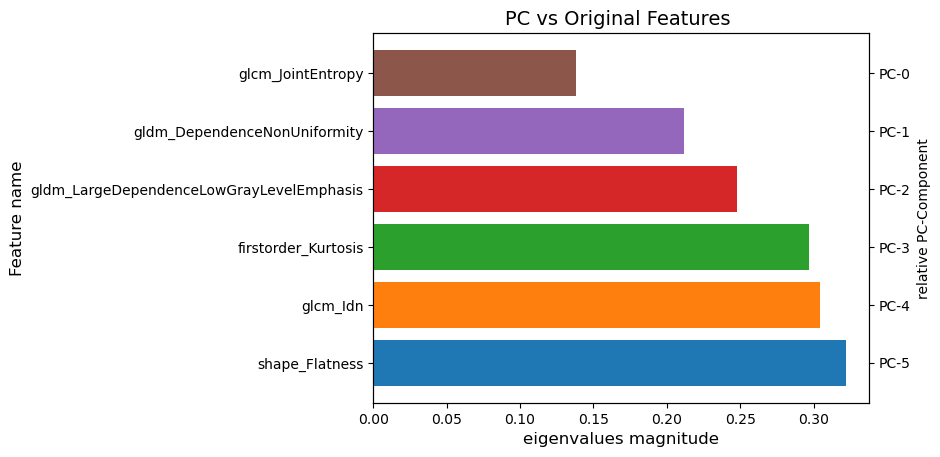
\includegraphics[width=\textwidth]{../images/importance.png}

    \caption{For each principal component (on the right), you can see which is the original feature (on the left)  that contributes more to the relative principal component.}
    \label{importance}
    
    \end{figure}


\begin{figure}[htp]

    \centering
    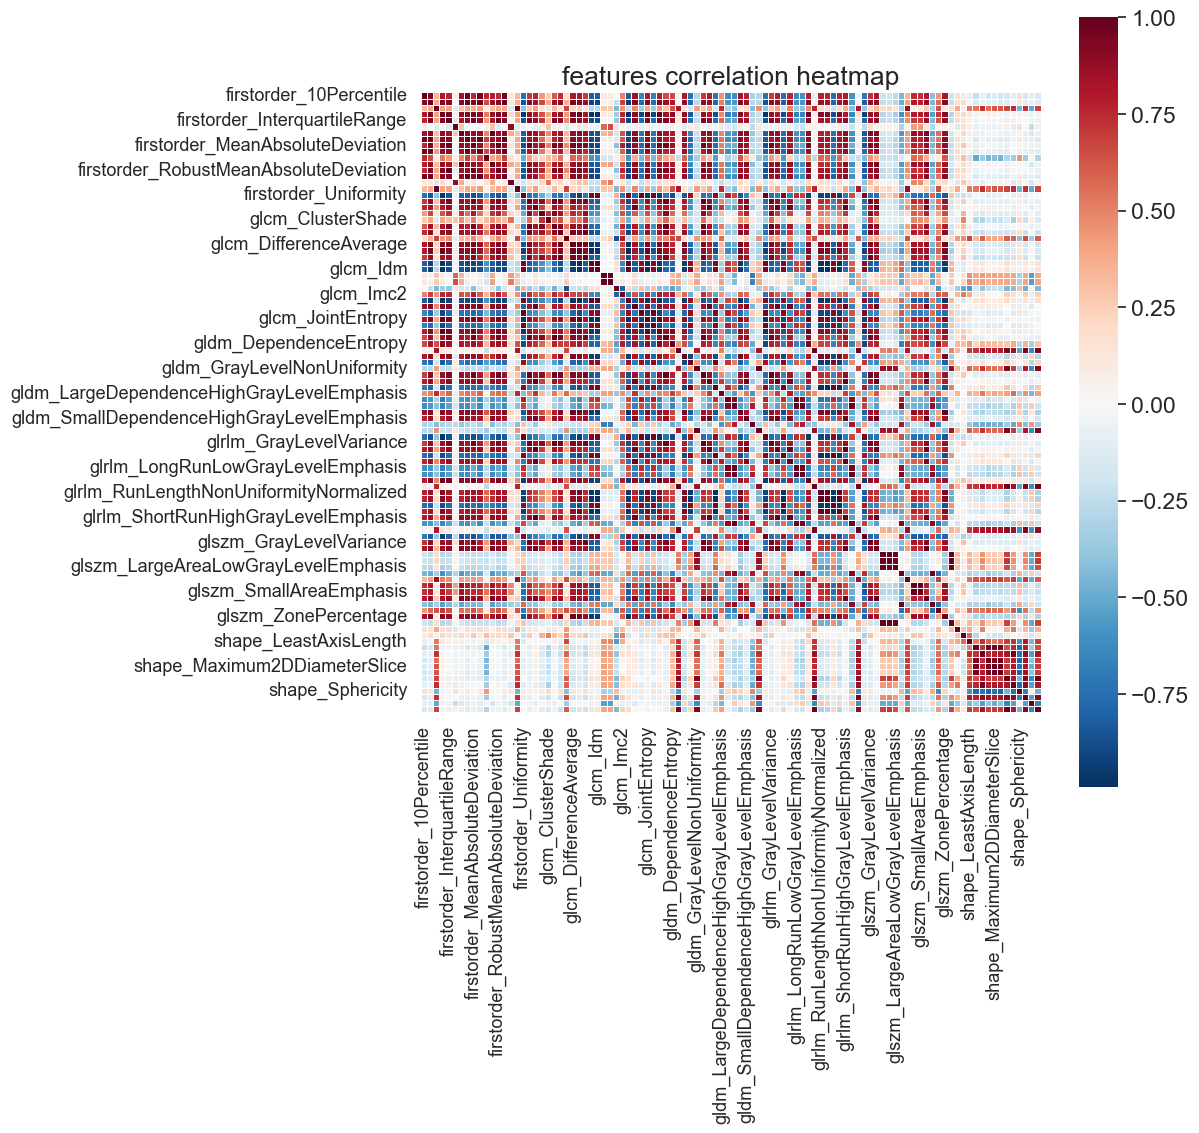
\includegraphics[width=0.99\textwidth]{../images/heatmap.png}

    \caption{Features correlation heatmap. The red color indicates a correlation, the white color indicates no correlation and the blue color indicates anti-correlation between features. \textit{Notes:} not every feature name has been plotted since 100 features caused the font size to be too small.}
    \label{heatmap}
    
    \end{figure}


\end{document}
\clearpage
\newpage
            % PREDICTION OF RESPONSE
            \documentclass{standalone}
\begin{document}
\subsection{Prediction of Response}

The prediction of response is based on the Tumor Regression Grade (TRG) which indicates the degree of response to neoadjuvant therapy\cite{tesicoppola}. TRG ranges from 0 to 5, resulting in a different response. Lower is the TRG higher the response. 
\\
To obtain the prediction of response, a custom Support Vector Classifier (SVC) model has been implemented.
The classification is made after the standardization and PCA performed as described before.
\\
The performed steps are:

\begin{itemize}
    \item Standardization of the data
    \item PCA 
    \item Classification
\end{itemize}

Unfortunately, not for every patient, the TRG was registered in the clinical database provided by the IRCCS Sant'Orsola-Malpighi Policlinic, so patients without it were excluded from the analysis.
Moreover, since the lack of data TRG values were binarized into two main classes: 0 and 1.
Class 0 means a complete response to the neoadjuvant chemo-radiotherapy (TRG values $ \in [0, \: 1])$ while class 1 means a moderate response (TRG values $ \in [2, \: 3])$ .
In Figure \ref{classesdistrib} you can see the distribution of the two classes.

\begin{figure}[ht]

    \centering
    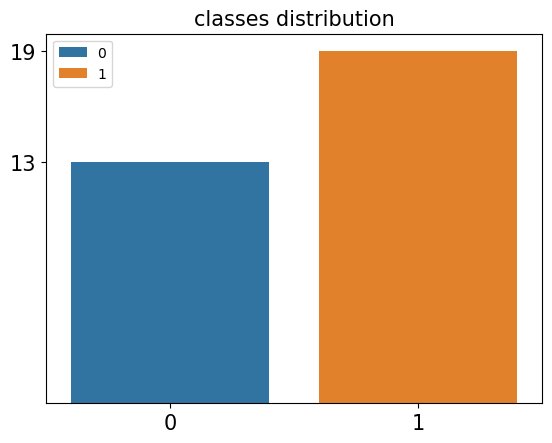
\includegraphics[width=0.52\textwidth]{../images/classesdistrib.png}

    \caption{Distribution of the classes. Class 0 means a complete response to the neo-adjuvant chemo-radiotherapy (TRG values $ \in [0, \: 1])$ while class 1 means a moderate response (TRG values $ \in [2, \: 3])$ }
    \label{classesdistrib}
    
    \end{figure}




\end{document}
\newpage
       % IMPLEMENTATION
       \documentclass{standalone}
\begin{document}
\section{Implementation}

I have implemented the pipeline described before using python, which is an high level object oriented programming language. 
The supported python versions are: $3.6| 3.7| 3.8| 3.9$.
To perform operations on images (image filtering, input-output operations, etc\dots), I've used different libraries depending on the specific purpose, as as anticipated in the description section.
\\
The whole code is open-source and available on GitHub \cite{img-segm} and the relative documentation, made using Sphinx, is available at : \url{https://img-segm.readthedocs.io/en/latest/?badge=latest}.
The installation is managed by setup.py, which also provides the full list of dependencies.
The pipeline installation is tested on MacOS (base environment) and on Linux by using the TravisCI host.
\\
The pipeline implementation provides also modules that allow one to load, visualize, processing the DICOM series and to train a U-Net model and scripts that provide a fast way to handle DICOM series and ROI from command line. 
\\
The detailed description of each module and script is available on GitHub.
Once you have installed it, you can start to segment the images directly from your bash, passing as input the path of the directory containing the DICOM series, to obtain the prediction of response.
\\
There are different output options that will be described in the results chapter.\\
This section will be aimed to show the implementation of the main steps of the described pipeline.

\end{document}

            % PRE-PROCESSING
            \documentclass{standalone}
\begin{document}
\subsection{Pre-processing}

As we said in the Description section, the pre-processing consists of the application of a smoothing filter and a gamma correction.
Before the processing operations, for each patient, the images needed to be read from the DICOM files as an array of pixels in order to apply the pre-processing functions.
This was done by the function $\mathtt{get\_slices}$: 

\begin{lstlisting}[language = python, caption=$\mathtt{get\_slices}$ implementation]
import numpy as np 
import pyradiomics

def read_slices(filename):

    _, ext = filename.split(".")

    if ext != "dcm":
        raise ValueError("Input filename must be a DICOM file")

    pix_arr = pydicom.dcmread(filename).pixel_array

    return pix_arr

def get_slices(dir_path)

    files = glob.glob(dir_path + "/*.dcm")

    # ordering as istance number
    z = [float(pydicom.read_file(f, force=True).get(
        "InstanceNumber", "0") - 1) for f in files]
    order = np.argsort(z)
    files = np.asarray(files)[order]

    slices = [read_slices(f) for f in files]
    slices = np.asarray(slices)

    return slices

\end{lstlisting}

For this purpose, I used the \textsc{Numpy} \cite{Numpy} and \textsc{Pydicom} \cite{Pydicom} libraries.
In particular, \textsc{Pydicom} provided functions to read DICOM files as pixel arrays and to access the \textit{InstanceNumber} (the current slice number stored in the header), while \textsc{Numpy} provided functions to sort the slices \textit{InstanceNumber} and get the images as an array of shape: (depth, height, width) where depth is the number of slices and (height, width) the image size.
\\
Once the images have been obtained, I could perform the steps described in the Description section:
\begin{itemize}
    \item normalization and rescaling
    \item denoising
    \item gamma correction
\end{itemize}

For this purpose, I used the \textsc{OpenCV} \cite{opencv_library} and \textsc{Scikit-Image} \cite{scikit-image} libraries:

\begin{lstlisting}[language = python, caption=pre-processing function implementation]
import cv2
from skimage.restoration import denoise_nl_means, estimate_sigma

def rescale(img):
    rescaled = cv2.normalize(img, dst=None, alpha=0, beta=1, norm_type=cv2.NORM_MINMAX, dtype=cv2.CV_32F)
    return rescaled


def denoise(img, alpha=10):

    patch_kw = dict(patch_size=5, patch_distance=6,)
    sigma_est = np.mean(estimate_sigma(img))
    denoised = denoise_nl_means(img, h=alpha * sigma_est, sigma=sigma_est, fast_mode=True, **patch_kw)
    return denoised


def gamma_correction(img, gamma=1.0):
    igamma = 1.0 / gamma
    imin, imax = img.min(), img.max()

    img_c = img.copy()
    img_c = ((img_c - imin) / (imax - imin)) ** igamma
    img_c = img_c * (imax - imin) + imin
    return img_c



def pre_processing_data(slices, alpha=10):

    imgs = []
    for layer in range(slices.shape[0]):
        img = slices[layer, :, :]
        if slices.shape[1:3] != 512:
            resized = cv2.resize(img, (512, 512))
        else:
            resized = img
        rescaled = rescale(resized)
        denoised = denoise(rescaled, alpha)
        gamma = gamma_correction(denoised)
        imgs.append(gamma)

    images = [np.expand_dims(im, axis=-1) for im in imgs]
    images = np.array(images)

    return images

\end{lstlisting}

In particular, the $\mathtt{rescale}$ function is used for the normalization and the rescaling of the images to binary floating-point 32-bit; the $\mathtt{denoise}$ function is used for the denoising process exploiting the \textsc{Scikit-Image} library; the $\mathtt{gamma\_correction}$ function is used for the gamma correction, thus increase/decrease the brightness of the image, depending on gamma.
All these three functions have been put together into $\mathtt{pre\_processing\_data}$ with a silent check on the image size, to get a single-shot pre-processing function.
The final output is an array, like $\mathtt{slices}$, containing the relative pre-processed images.

\end{document}

            % TRAINING AND SEGMENTATION
            \documentclass{standalone}
\begin{document}
\subsection{Training and Segmentation}

Training a was performed using \textsc{TensorFlow}\cite{Tensorflow} and \textsc{Segmentation-models} API\cite{segmentation_models}.
The core of the training process is the custom $\mathtt{DataGenerator}$, which provides data, split them into training and validation set, perform pre-processing and data augmentation on the training set.
The peculiarity consists of the capability of working directly with DICOM input files.
The input and label images are taken directly by the $\mathtt{DataGenerator}$, providing the relative $\mathtt{source\_path}$ and $\mathtt{label\_path}$ that are the paths of the directories containing the relative DICOM input and labels images.

\begin{lstlisting}[language = python, caption=Custom $\mathtt{DataGenerator}$ implementation]
import tensorflow as tf
import pyradiomics
    
class DataGenerator:

    def __init__(self, batch_size, source_path, label_path, aug=False, seed=123, validation_split=0., subset='training'):


        np.random.seed(seed)
        source_files = sorted(glob.glob(source_path + '/*.dcm'))
        source_files = np.asarray(source_files)


        labels_files = sorted(glob.glob(label_path + '/*.png'))
        labels_files = np.asarray(labels_files)

        assert source_files.size == labels_files.size


        source_files, labels_files = self.randomize(source_files, labels_files)

        idx = np.arange(0, source_files.size)
        np.random.shuffle(idx)

        self._source_trainfiles = source_files[idx[int(source_files.size * validation_split):]]
        self._labels_trainfiles = labels_files[idx[int(labels_files.size * validation_split):]]

        self._source_valfiles = source_files[idx[:int(source_files.size * validation_split)]]
        self._labels_valfiles = labels_files[idx[:int(labels_files.size * validation_split)]]

        self.subset = subset

        if self.subset == 'training':
            self._num_data = self._source_trainfiles.size
        elif self.subset == 'validation':
            self._num_data = self._source_valfiles.size

        self.aug = aug
        self._batch = batch_size
        self._cbatch = 0
        self._data, self._label = (None, None)

    @property
    def num_data(self):
        return self._num_data

    def randomize(self, source, label):

        random_index = np.arange(0, source.size)
        np.random.shuffle(random_index)
        source = source[random_index]
        label = label[random_index]

        return (source, label)


    def resize(self, img, lbl):

        height, width = img.shape[0], img.shape[1]

        if height != 512:
            img = cv2.resize(img, (512, 512))
            lbl = cv2.resize(lbl, (512, 512))
        else:
            img = img
            lbl = lbl

        return (img, lbl)

    def random_vflip(self, img, lbl):
        idx = np.random.uniform(low=0., high=1.)
        if idx > 0.5:
            return (cv2.flip(img, 0), cv2.flip(lbl, 0))
        else:
            return (img, lbl)

    def random_hflip(self, img, lbl):
        idx = np.random.uniform(low=0., high=1.)
        if idx > 0.5:
            return (cv2.flip(img, 1), cv2.flip(lbl, 1))
        else:
            return (img, lbl)

    def rescale(self, img):
        rescaled = cv2.normalize(img, dst=None, alpha=0, beta=1, norm_type=cv2.NORM_MINMAX, dtype=cv2.CV_32F)
        return rescaled

    def denoise(self, img):

        patch_kw = dict(patch_size=5, patch_distance=6)
        sigma_est = np.mean(estimate_sigma(img))
        denoised = denoise_nl_means(img, h=10 * sigma_est, sigma=sigma_est, fast_mode=True, **patch_kw)
        return denoised

    def gamma_correction(self, img, gamma=1.0):
        igamma = 1.0 / gamma
        imin, imax = img.min(), img.max()

        img_c = img.copy()
        img_c = ((img_c - imin) / (imax - imin)) ** igamma
        img_c = img_c * (imax - imin) + imin
        return img_c

    def __iter__(self):
        self._cbatch = 0
        return self

    def __next__(self):
        if self._cbatch + self._batch >= self._num_data:
            self._cbatch = 0
            self._source_trainfiles, self._labels_trainfiles = self.randomize(self._source_trainfiles, self._labels_trainfiles)
            self._source_valfiles, self._labels_valfiles = self.randomize(self._source_valfiles, self._labels_valfiles)

        if self.subset == 'training':
            c_sources = self._source_trainfiles[self._cbatch:self._cbatch + self._batch]
            c_labels = self._labels_trainfiles[self._cbatch:self._cbatch + self._batch]
        elif self.subset == 'validation':
            c_sources = self._source_valfiles[self._cbatch:self._cbatch + self._batch]
            c_labels = self._labels_valfiles[self._cbatch:self._cbatch + self._batch]

        # load the data

        images = [pydicom.dcmread(f).pixel_array for f in c_sources]
        labels = [cv2.imread(f, 0) for f in c_labels]


        # check size

        images, labels = zip(*[self.resize(im, lbl) for im, lbl in zip(images, labels)])

        # cast

        images = [self.rescale(im) for im in images]
        labels = [self.rescale(lbl) for lbl in labels]

        # denoise
        images = [self.denoise(im) for im in images]

        # gamma correction
        images = [self.gamma_correction(im, gamma=1.5) for im in images]

        if self.aug:

            # random horizontal flip
            images, labels = zip(*[self.random_hflip(im, lbl) for im, lbl in zip(images, labels)])

            # random vertical flip
            images, labels = zip(*[self.random_vflip(im, lbl) for im, lbl in zip(images, labels)])

        images = [im[..., np.newaxis] for im in images]
        labels = [lbl[..., np.newaxis] for lbl in labels]

        # to numpy

        images = np.array(images)
        labels = np.array(labels)

        self._cbatch += self._batch

        return (images, labels)

    
\end{lstlisting}
The model and the losses used for the training, come from \textsc{Segmentation-models} API.
In particular, the model consists of a U-net architecture using \textit{efficientnetb0} as
backbone encoder.
The metric instead, $\mathtt{dice\_coeff}$, has been implemented by using \textsc{TensorFlow} functions.

\begin{lstlisting}[language = python, caption=model implementation]
import tensorflow as tf
import segmentation_models as sm

BACKBONE = 'efficientnetb0'
model = sm.Unet(BACKBONE, input_shape=(IMAGE_HEIGHT, IMAGE_WIDTH, 1), encoder_weights=None, activation='sigmoid')

optimizer =  'adam'
    
dice_loss = sm.losses.DiceLoss()
focal_loss = sm.losses.BinaryFocalLoss()
loss = dice_loss + (1 * focal_loss)

def dice_coef(y_true, y_pred):
    intersection = tf.reduce_sum(y_true * y_pred, axis=[1, 2, 3])
    total = tf.reduce_sum(y_true, axis=[1, 2, 3]) + tf.reduce_sum(y_pred, axis=[1, 2, 3])
    dice = tf.reduce_mean((2. * intersection + smooth) / (total + 1.))
    return dice

metrics = [ dice_coef ]

model.compile(optimizer=optimizer, loss=loss, metrics=metrics)

\end{lstlisting}
The prediction of the images is obtained using the function $\mathtt{predict\_images}$,
providing the $\mathtt{slices}$ and the trained model. 
The result is an array, like $\mathtt{slices}$, containing the relative prediction for each slice.
\begin{lstlisting}[language = python, caption=prediction function implementation]

def predict_images(slices, model, pre_processing=False, t=0.1):

    if pre_processing:
        prep_slices = pre_processing_data(slices)
    else:
        prep_slices = slices

    predicted_slices = np.zeros_like(prep_slices)

    for layer in range(slices.shape[0]):
        img = prep_slices[layer, ...]
        predicted_slices[layer, ...] = model.predict(img[np.newaxis, ...])[...]
        predicted_slices[layer, ...] = np.where(predicted_slices[layer, ...] <= 0.1, 0, predicted_slices[layer, ...])


    return predicted_slices


\end{lstlisting}



\end{document}

            % FEATURES EXTRACTION AND ANALYSIS
            \documentclass{standalone}
\begin{document}
\subsection{Features Extraction and Analysis}

For this purpose, I used the \textsc{Pyradiomics} library\cite{Pyradiomics} to extract features from each single slice of the patient after storing for each patient input and segmented images as 3D images (.nrrd format) in a dedicated directory, using \textsc{SimpleITK} library \cite{SimpleITK}, required by \textsc{Pyradiomics}. 
From each patient a total of 100 radiomic features were extracted.
The extraction settings were stored in a $\mathtt{Params.yaml}$ file required by \textsc{Pyradiomics}.
\begin{lstlisting}[language = python, caption=Features extraction implementation]
from radiomics import featureextractor
import pandas as pd
import numpy as np
import SimpleITK as sitk

params  = '../extras/Params.yaml'
extractor = featureextractor.RadiomicsFeatureExtractor(params)

features = {}

for patient in good_patients:

    dirs = glob.glob(src + '/' + patient + '/*_NRRD')
    
    
    for directory in dirs:

        original = sitk.ReadImage(directory + "/original.nrrd")
        segmented = sitk.ReadImage(directory + "/segmented.nrrd")

        folder_name = os.path.split(directory)[1]
        fold_prefix = folder_name.split('_')[0]

        features[patient, fold_prefix] = extractor.execute(original, segmented)

    
\end{lstlisting}

Features are stored in a dictionary, which the key is the caseID of patient and the the name of the examination directory containing the dicom series.
I started to visualize and sort the features for each patient and stored them into a pandas Dataframe $\mathtt{df}$ made by 100 columns (one for each extracted feature) and the number of rows made by the number of patients.

\begin{lstlisting}[language = python, caption=Features dataframe implementation]

dict_list = list(features)
feature_names = list(sorted(filter ( lambda k: k.startswith("original_"), features[dict_list[0]] )))

print('NUMEBR OF CASE_ID: ', len(dict_list))
print('NUMEBR OF FEATURES: ', len(feature_names))
print(dict_list)

sorted_list = sorted(dict_list, key=lambda x: int(x[0].replace('BO', '')))


sorted_ID = list(map(lambda x: x[0], sorted_list))

samples = np.zeros((len(sorted_list), len(feature_names)))

for k, case_id in enumerate(sorted_list):
    a = np.array([])
    for feature_name in feature_names:
        a = np.append(a, features[case_id][feature_name])
    samples[k, ...] = a

#for possible NaNs
samples = np.nan_to_num(samples)

samples.shape

df = pd.DataFrame(data=samples, columns=feature_names, index=sorted_ID)

        
\end{lstlisting}

Then, I uploaded the database containing clinical data to access the Tumor Regression Grade (TRG) values.
Unfortunately, not for every patient data were available, so the patients rows without TRG values were dropped, thus excluded from the analysis.
To overcome the lack of data, TRG values were binarized.
In order to reduce features, PCA was performed setting $\mathtt{n\_components = .9}$ (meaning the number of components that gives the $90 \%$ of the toal variance) by using \textsc{Scikit-learn} library\cite{scikit}, exploiting $\mathtt{make\_pipeline}$ to standardize data before the PCA.
Then, thanks to the attribute $\mathtt{components\_}$ , that outputs an array of shape $[ \mathtt{n \_ components} , \:  \mathtt{n \_ features} ]$, it is possible to get how components are related to the original features.

\begin{lstlisting}[language = python, caption=PCA implementation]
from sklearn.preprocessing import StandardScaler
from sklearn.decomposition import PCA
from sklearn.pipeline import make_pipeline

clinical_df = pd.read_excel('../data/clinical_db.xlsx', sheet_name='data', index_col='PatientID')

TRG = clinical_df['TRG']

df = pd.concat([df, TRG], axis=1)
df = df[df['TRG'].notna()]


X = df.drop('TRG', axis=1)
y = df['TRG'].values
y = np.where(y <=1, 0, 1)

pca = make_pipeline(StandardScaler(), PCA(n_components=.9, svd_solver='full'))
pca.fit(X, y)


print(pd.DataFrame(pca.components_,columns=X.columns, index = ['PC-0','PC-1', 'PC-2', 'PC-3', 'PC-4', 'PC-5']))
\end{lstlisting}




\end{document}

            % PREDICTION OF RESPONSE
            \documentclass{standalone}
\begin{document}
\subsection{Prediction of Response}

This step was implemented exploiting $\mathtt{make\_pipeline}$ to get the prediction of response after scaling and performing PCA.
The prediction is given by a Support Vector Classifier $\mathtt{SVC}$, setting the parameter $C = 100$.
Cross validation was performed exploiting $\mathtt{cross\_val\_predict}$ and $\mathtt{StratifiedKFold}$ of the \textsc{Scikit-learn} library\cite{scikit}.
In particular, to get the $\mathtt{random\_state}$ of the $\mathtt{StratifiedKfold}$ was set to the median value of the Matthews Correlation coefficient distribution, obtained after 500 simulations.
Finally the classification report was provided by using the $\mathtt{classification\_report}$ of \textsc{Scikit-learn}.


\begin{lstlisting}[language = python, caption=Prediction of response implementation]
from sklearn.preprocessing import StandardScaler
from sklearn.decomposition import PCA
from sklearn.pipeline import make_pipeline
from sklearn.model_selection import cross_val_predict, StratifiedKFold
from sklearn.svm import SVC
from sklearn.metrics import matthews_corrcoef
from sklearn.metrics import classification_report
    
X = df.drop('TRG', axis=1)
y = df['TRG'].values
y = np.where(y <=1, 0, 1)

pipeline = make_pipeline(StandardScaler(), PCA(n_components=.9, svd_solver='full'), SVC(C=100, probability=True, random_state=0))

n_splits = 10

M_coeffs = []
for i in range(500):
    skf = StratifiedKFold(n_splits=n_splits, shuffle=True, random_state=i + 1)
    y_pred = cross_val_predict(pipeline, X, y, cv=skf)
    MCC = matthews_corrcoef(y, y_pred)
    #M_coeffs[i] = MCC
    M_coeffs.append(MCC)

data = M_coeffs
median = np.argsort(data)[len(data)//2]
print(median)
data[median]

skf = StratifiedKFold(n_splits=n_splits, shuffle=True, random_state=median + 1)
y_pred = cross_val_predict(pipeline, X, y, cv=skf)

target_names = ['class 0', 'class 1']
print(classification_report(y, y_pred, target_names=target_names))



\end{lstlisting}
    

\end{document}
            
\end{document}
\documentclass{standalone}
\begin{document}

    % INTRO
    \documentclass{standalone}
\begin{document}
\chapter{Results}
This Chapter will be aimed to show and discuss the results of the developed pipeline.
First of all, a brief description of the Dataset provided by the IRCCS Sant’Orsola-Malpighi Policlinic will be provided.
Then, the accuracy of the segmentation and of the prediction of response.
Finally, the outputs of the implementation will be shown.

\end{document}

        % DATASET DESCRIPTION
        \documentclass{standalone}
\begin{document}
\section{Dataset Description}
The main dataset used for this project was provided by IRCCS Sant’Orsola-Malpighi Polyclinic.
It consists of MRI from 48 patients affected by colorectal cancer undergoing neo-adjuvant radio-chemotherapy, from January 2018 to the end of December 2019.
The scans are provided slice by slice in DICOM format.
The scans are T2-weighted images resulting in images that highlight fat (low signal) and water (high signal) within the body.
Within the scans, also manual annotations, made by expert clinicians, were provided.
The medical annotations consist of sets of $(x, y)$ points that border the tumor area on the relative image.
Clinical data were also provided through a dedicated database.
Among the information stored, the clinical database contains the Tumor Regression Grade (TRG) which indicates the degree of response to neoadjuvant therapy.

\begin{table}[ht]
	\centering
	\begin{tabular}{lc}
		\toprule
		\textbf{Property} & \textbf{Value}   \\
	    \midrule
		Number of patients &  48 \\
	    \midrule
		Distribution by sex (M/F) &  29/19 \\
		\midrule
		Distribution by age (min/median/max) &   48/70/89  \\
		\bottomrule
	\end{tabular}
	\caption{Dataset properties.}
	\label{tab:properties}
\end{table}


\end{document}
\newpage
        % ACCURACY
        \documentclass{standalone}
\begin{document}
\section{Performance}
In this section, I will show the results of the accuracy achieved by the implemented pipeline.
The segmentation performance has been evaluated since the training process and the obtained results are compared with the literature.
A comparison between the results of segmentation and the medical annotation (ground-truth) will be also provided.
\\
The accuracy for the prediction of response has been measured by using dedicated metrics.
\end{document}
                % SEGMENTATION
                \documentclass{standalone}
\begin{document}
\subsection{Segmentation}

The metric used for checking the performance of the segmentation results is given by the Dice Similarity Coefficient (DSC) evaluated on the validation set.
This is because it was the most used in literature for this purpose and so for make it possible results comparison.
The total number of involved patients lowered from 48 to 37 because of misregistration between images and medical annotations for some of them.
The training process was performed for 150 epochs\footnote{The term epoch indicates the number of passes of the entire training dataset the machine learning algorithm has completed.} on 391 images (training set) and validated on 97 images (validation set).
The Training process took almost 7 hours, on the new Apple Silicon M1 Macbook Pro equipped with 8 GB of RAM.
The results of the training process can be seen in Figure \ref{training}.
The plots show the curves for the model dice coefficient and the model loss as a function of the epochs.
In particular, the blue curve represents the results obtained for the training set of data while the green one represents the results obtained for the validation set.
\\
In Table \ref{results}, you can see the comparison between the state of the art and the implemented pipeline about colorectal cancer segmentation.
We must remember that the literature about MRI colorectal cancer segmentation performed by using CNNs, unlike other topics, is not very wide.
However, it comes out that automatic segmentation is quite hard to perform on Magnetic Resonance colorectal cancer images due to different issues: data; medical annotations; loss function.
In fact, as showed by Jovana Panic at al.\cite{jpanic} mucinous cases can considerably affect the performances.
Moreover, the performance can be affected by how medical annotations are made.
Trebeschi et al. \cite{Trebeschi2017} showed that the DSC of the same model trained using medical annotations made by different experts can give different DSC scores.
Another sensitive factor is the loss function. 
As shown by Yi. Jie Huang et al.\cite{YiJieHuang}, depending on the network's architectures and the loss functions you can have different performances. 
 
\begin{table}[ht]
	\Large
	\centering
	\resizebox{\textwidth}{!}{\begin{tabular}{p{4.8cm}p{4.6cm}p{4.9cm}p{5cm}p{4.9cm}} \toprule
		{\textbf{Trebeschi et al.}} & {\textbf{Panic et al.}} & {\textbf{Yi-Jie Huang et al.}} & {\textbf{Xiaoling Pang et al.}} & {\textbf{Implemented pipeline}} \\ \midrule
		DSC= 0.68  & DSC = 0.58   &  DSC = $[0.66 - 0.72]$  &  DSC = 0.66 &  \textbf{DSC = 0.71} \\
		DSC= 0.70&   &  & &   \\
		\midrule
		140 patients &  33 patients & 64 cancerous cases & 275 patients & \textbf{37 patients}  \\
			& (5 mucinous cases)  &  & excluding mucinous  & \textbf{including some }  \\
			&   &  & cases  & \textbf{mucinous cases}    \\
	\midrule
	Custom Network  &   Custom Network  & Custom network  & U-net & \textbf{U-net, backbone} \\
	architecture & architecture  &  architectures &   &  \textbf{EfficientNetb0}  \\
	\bottomrule
	\end{tabular}}

	\caption{Results comparison between state-of-art and the implemented pipeline about MRI colorectal cancer scans segmentation by using CNNs.}
	\label{results}
	
\end{table}


\begin{figure}[ht]

    \centering
    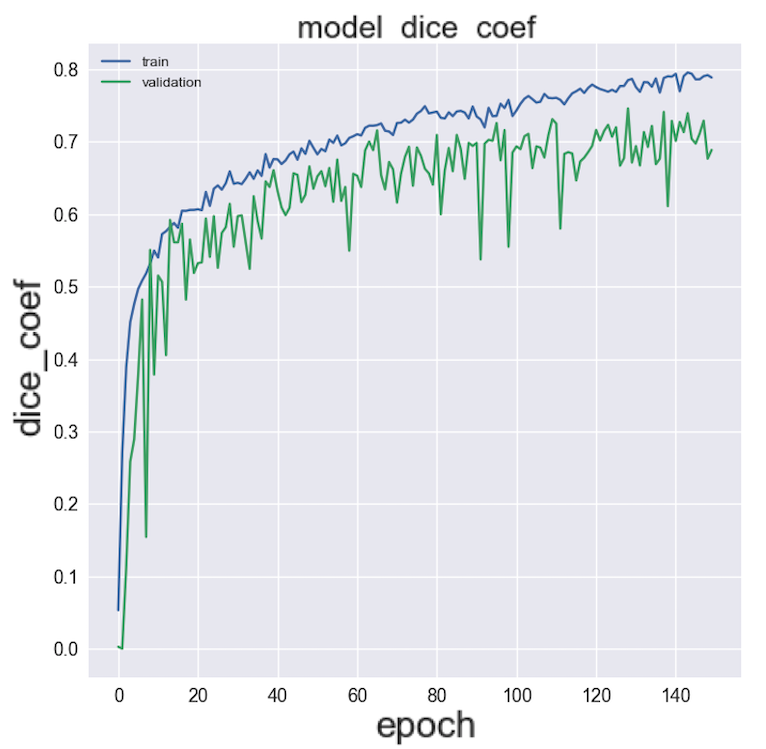
\includegraphics[width=0.49\textwidth]{../images/dice_coef.png}
	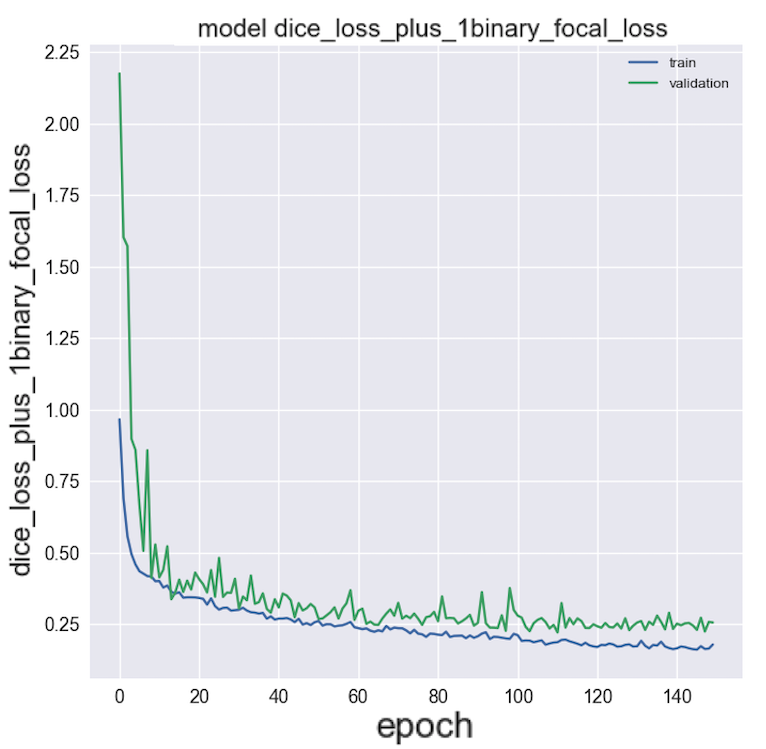
\includegraphics[width=0.49\textwidth]{../images/loss.png}

    \caption{Model history plots on training (blue) and validation (green) set. \textit{Left}): DSC as a function of the epochs. \textit{Right}): model loss as a function of the epochs.}
    \label{training}
    
\end{figure}
\clearpage
\newpage

\subsubsection{Comparison with Manual Annotations}


To check the pipeline performances, I have also compared the obtained segmentation with the manual annotation (Ground-truth) made by expert radiologists.
In Figure \ref{predtraining}, you can see the comparison for images belonging to the training set while in Figure \ref{predvalidation} the comparison for the ones belonging to the validation set.
The prediction is plotted as a probability density map between 0. and 1. as shown by the sequential colormap.
Both in Figure \ref{predtraining} and \ref{predvalidation}, I also included a case of \textit{mucinous} (first row), showing that the model is able to distinguish also this type of tumor, even if the contour is not as precise as the ground-truth one.
\\
Unfortunately, for a few cases, the model failed to segment correctly the right Region of Interest (ROI).
Some of this cases are shown in Figure \ref{predwrong}.
\\
The goodness of the comparison can also be appreciated from the comparison between the ground truth and the prediction over the original image.
In Figure \ref{predoverlaptraining} and \ref{predoverlaptraining2} the images belong to the training set while in Figure \ref{predoverlapvalidation} and \ref{predoverlapvalidation2} the images belong to the validation one.
Also for this case, the prediction is plotted as a probability density map between 0. and 1. as shown by the sequential colormap.


\begin{figure}[htp]

    \centering
    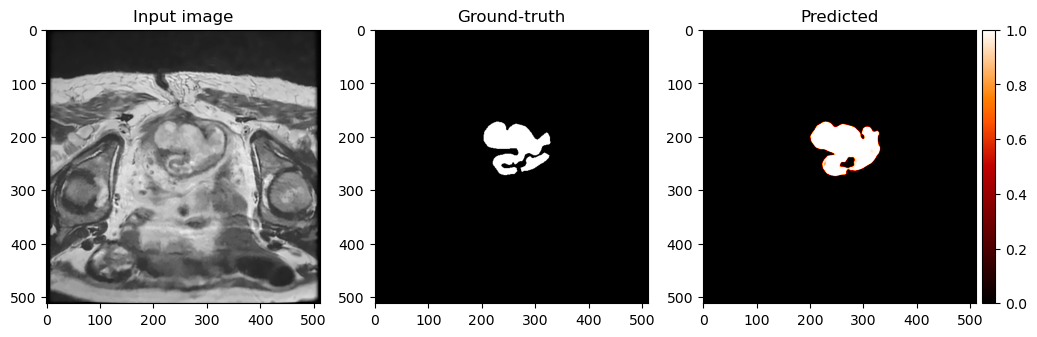
\includegraphics[width=\textwidth]{../images/predoutputr.png}
    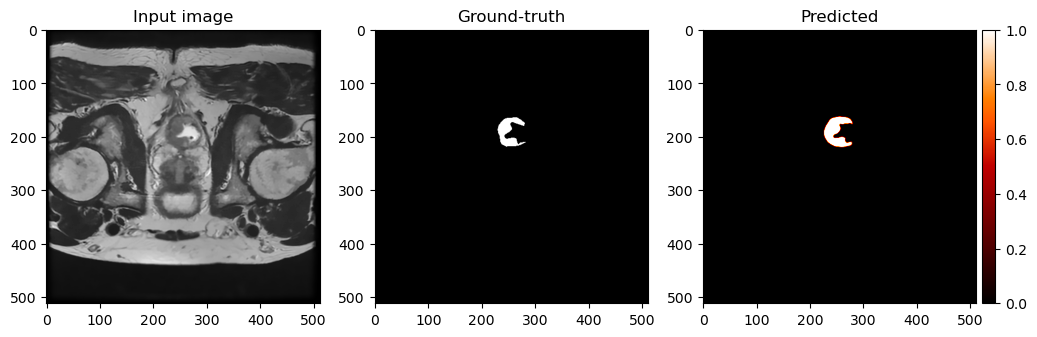
\includegraphics[width=\textwidth]{../images/predoutputr1.png}
    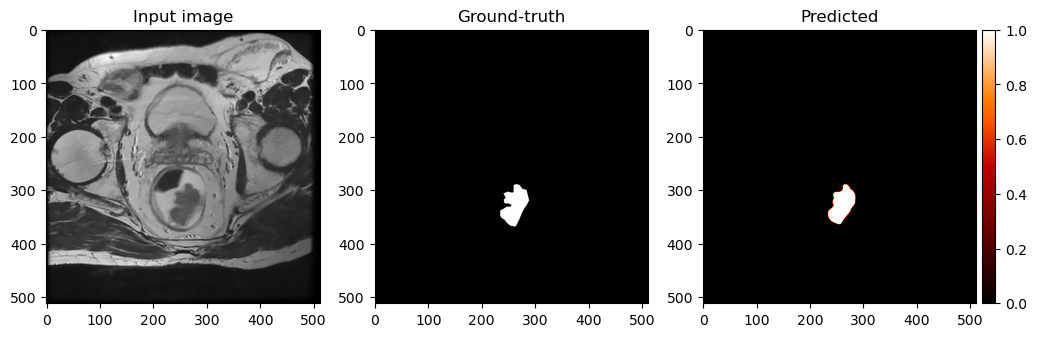
\includegraphics[width=\textwidth]{../images/predoutputr2.png}

    \caption{Comparison between the ground-truth image and the predicted one by the CNN model. The first column represents the input image. 
    The second one represents the ground-truth image. 
    Finally, the third one represents the predicted tumor area.
    The prediction is plotted as a probability density map between 0. and 1. as shown by the sequential colormap.
    From training set.}\label{predtraining}


\end{figure}



\begin{figure}[htp]

    \centering
    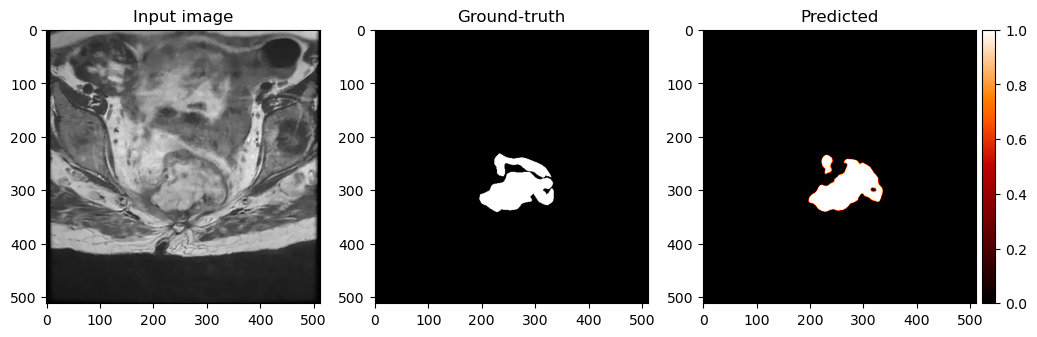
\includegraphics[width=\textwidth]{../images/predoutput2.png}
    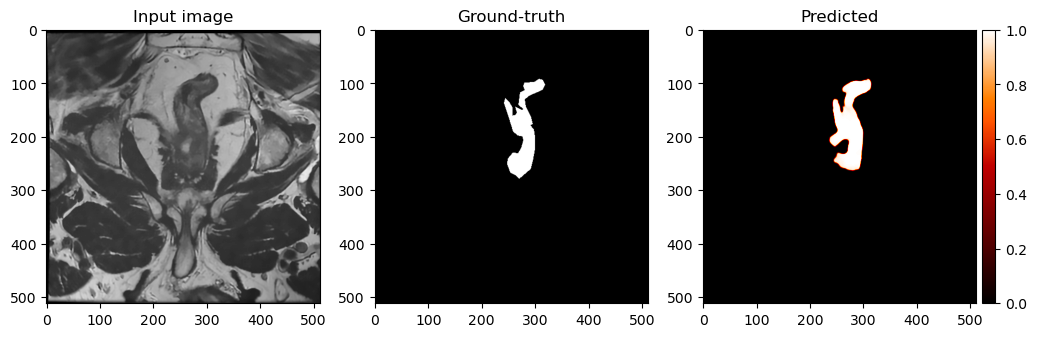
\includegraphics[width=\textwidth]{../images/predoutput.png}
    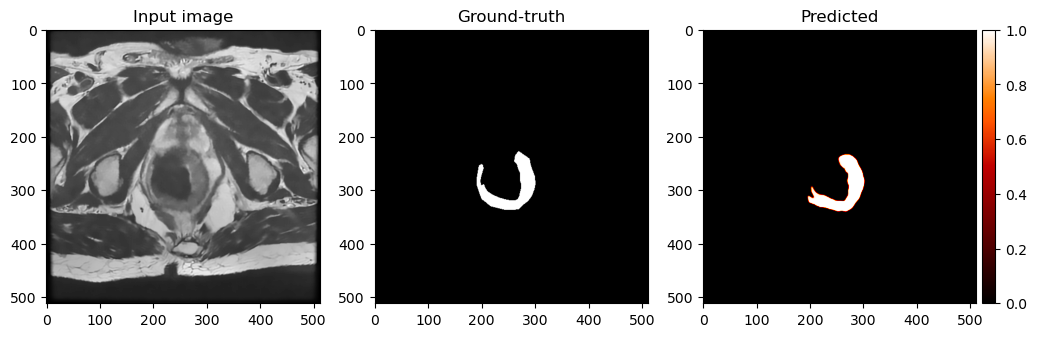
\includegraphics[width=\textwidth]{../images/predoutput1.png}
    

    \caption{Comparison between the ground-truth image and the predicted one by the CNN model. The first column represents the input image. 
    The second one represents the ground-truth image. 
    Finally, the third one represents the predicted tumor area.
    The prediction is plotted as a probability density map between 0. and 1. as shown by the sequential colormap.
    From validation set.}\label{predvalidation}

\end{figure}


\begin{figure}[htp]

    \centering
    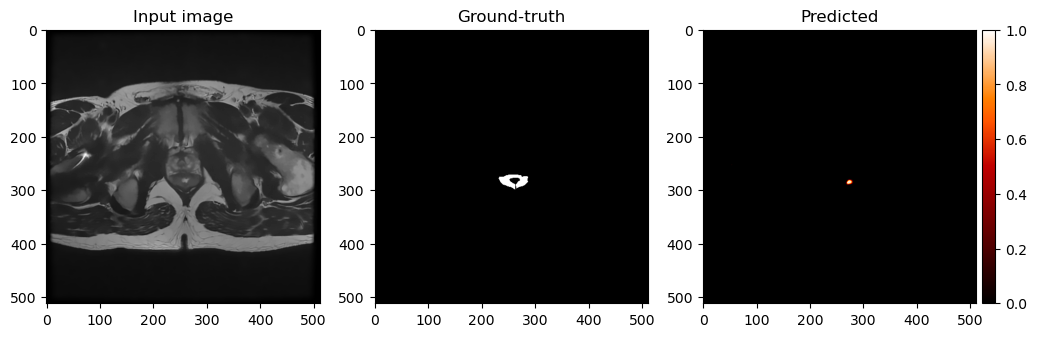
\includegraphics[width=\textwidth]{../images/predoutputwrong.png}
    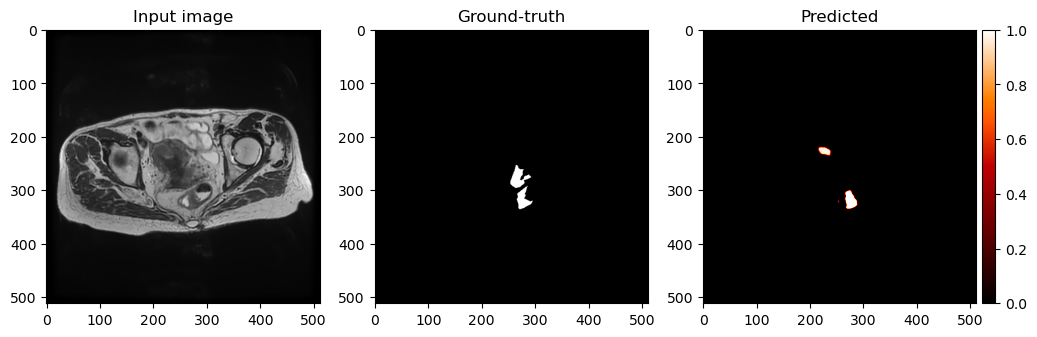
\includegraphics[width=\textwidth]{../images/predoutputwrong1.png}
    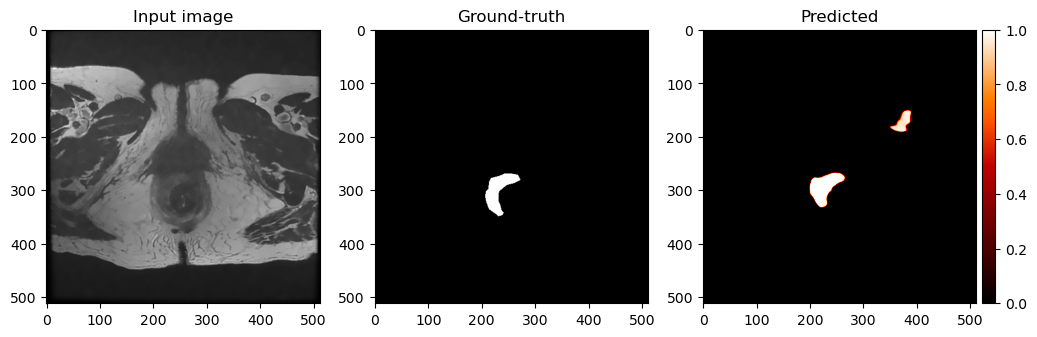
\includegraphics[width=\textwidth]{../images/predoutputwrong2.png}
    

    \caption{Comparison between the ground-truth image and the predicted one by the CNN model. The first column represents the input image. 
    The second one represents the ground-truth image. 
    Finally, the third one represents the predicted tumor area.
    The prediction is plotted as a probability density map between 0. and 1. as shown by the sequential colormap.
    Bad segmentation cases.}\label{predwrong}

\end{figure}


\begin{figure}[htp]

    \centering
    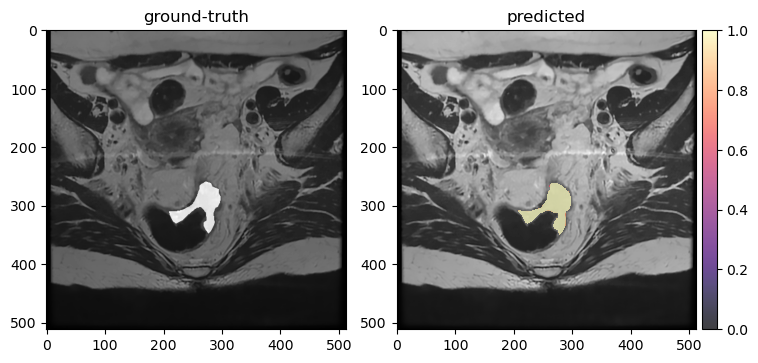
\includegraphics[width=\textwidth]{../images/predoutputoverlap2.png}
    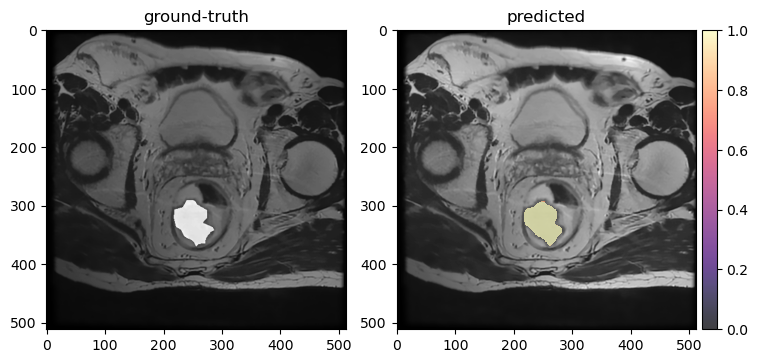
\includegraphics[width=\textwidth]{../images/predoutputoverlap1.png}
    
    \caption{Comparison between the ground-truth image and the prediction over the original image.
    The prediction is plotted as a probability density map between 0. and 1. as shown by the sequential colormap.
    From training set.}\label{predoverlaptraining}

\end{figure}

\begin{figure}[htp]

    \centering
    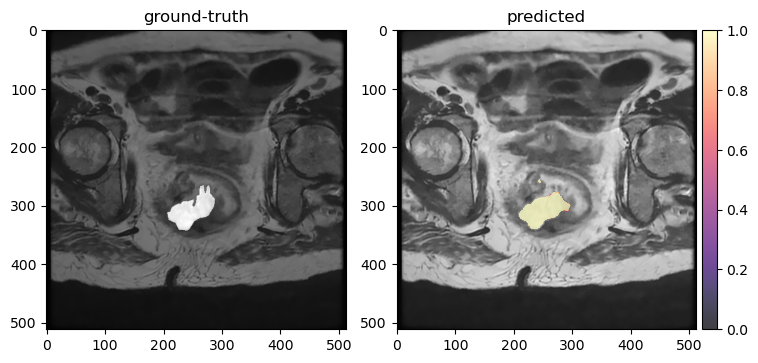
\includegraphics[width=\textwidth]{../images/predoutputoverlap3.png}
    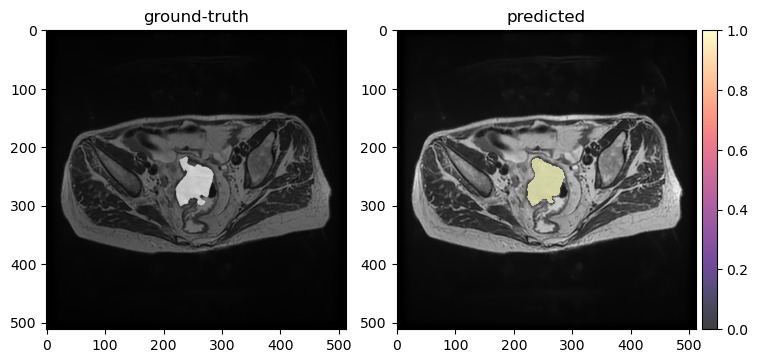
\includegraphics[width=\textwidth]{../images/predoutputoverlap4.png}
    
    \caption{Comparison between the ground-truth image and the prediction over the original image.
    The prediction is plotted as a probability density map between 0. and 1. as shown by the sequential colormap.
    From training set.}\label{predoverlaptraining2}

\end{figure}

\begin{figure}[htp]

    \centering
    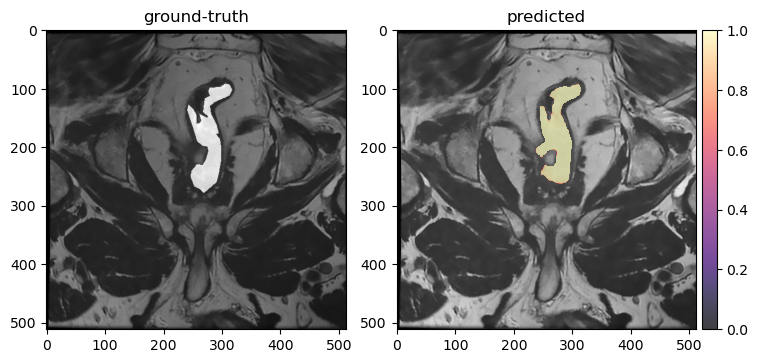
\includegraphics[width=\textwidth]{../images/predoutputoverlapvalidation.png}
    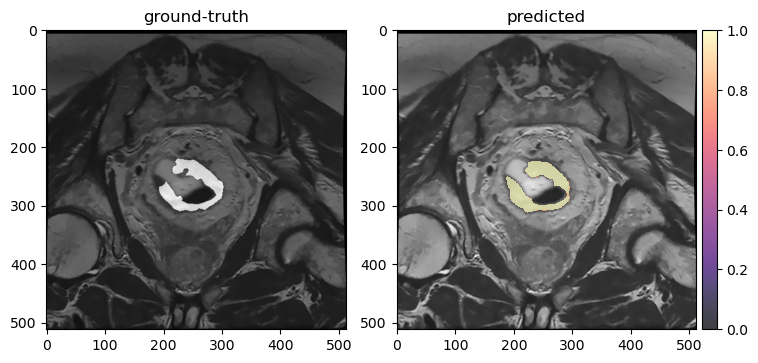
\includegraphics[width=\textwidth]{../images/predoutputoverlapvalidation1.png}
    
    
    \caption{Comparison between the ground-truth image and the prediction over the original image.
    The prediction is plotted as a probability density map between 0. and 1. as shown by the sequential colormap.
    From validation set.}\label{predoverlapvalidation}

\end{figure}


\begin{figure}[htp]

    \centering
    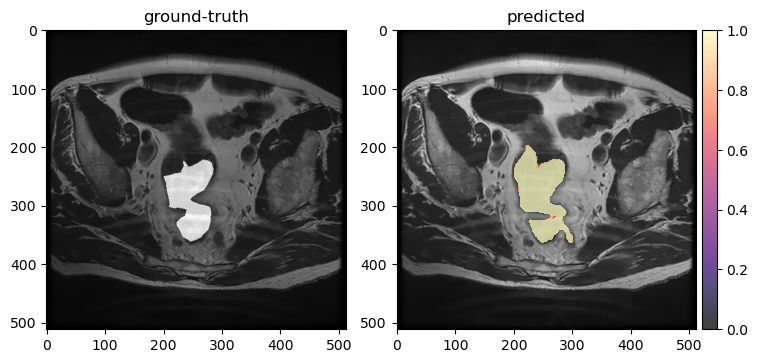
\includegraphics[width=\textwidth]{../images/predoutputoverlapvalidation2.png}
    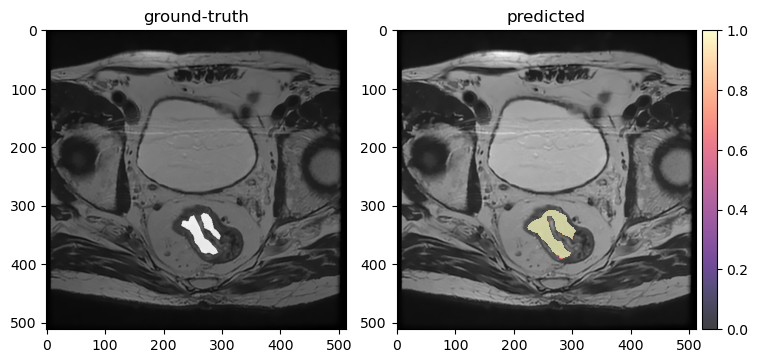
\includegraphics[width=\textwidth]{../images/predoutputoverlapvalidation3.png}
    
    
    \caption{Comparison between the ground-truth image and the prediction over the original image.
    The prediction is plotted as a probability density map between 0. and 1. as shown by the sequential colormap.
    From validation set.}\label{predoverlapvalidation2}

\end{figure}


\newpage
\end{document}

                % PRED OF RESP
                \documentclass{standalone}
\begin{document}
\subsection{Prediction of Response}

The accuracy for the prediction of response was measured by using different metrics.
\\
In Table \ref{tab:classreport} you can see the classification report made by the Precision, Recall, and F1 score for each class (Class 0 for complete response and Class 1 for moderate response).
\\
Unfortunately, the TRG value was missing for some patients, therefore some of them were excluded from the analysis.
In the end, the total number of patients was 32, that is the sum of the \textit{support} column values for Class 0 and Class 1.
\\
The classifier model was cross-validated to avoid the presence of \textit{bias} during the split into training and test set of the data on 500 simulations, evaluating the Matthews Correlation coefficient (MCC).
The result is a distribution of the MCC, that you can see in Figure \ref{MCC}, with a median $MCC=0.55$ .

\begin{table}[ht]
	\centering
	\begin{tabular}{ccccc}
		\toprule
		  & \textbf{Precision}  & \textbf{Recall} & \textbf{F1-Score} & \textbf{Support}\\
	    \midrule
		\textbf{Class 0} &  0.71 &  0.77 &  0.74 &  13\\
	    \midrule
		\textbf{Class 1} &  0.83 &  0.79 &  0.81 &  19\\
		\bottomrule
	\end{tabular}
	\caption{Classification report}
	\label{tab:classreport}
\end{table}



\begin{figure}[ht]

	\centering
	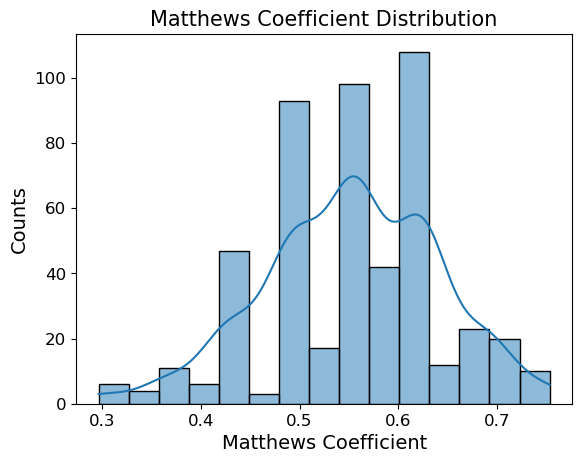
\includegraphics[width=0.65\textwidth]{../images/MCC.png}

	\caption{Matthews Correlation coefficient distribution for the pipeline obtained after 500 simulations.}
	\label{MCC}
	
	\end{figure}


\newpage
I also computed the confusion matrix , in Figure \ref{confmatrix}, to evaluate the accuracy of the classification.
For Class 0, so for a complete response, the well-classified instances are 10 over a total of 13, thus the wrong-classified ones are 3.
For Class 1, so for a moderate response, the well-classified instances are 15 over a total of 19, thus the wrong-classified ones are 4.


\begin{figure}[htp]

    \centering
    \includegraphics[width=0.8\textwidth]{../images/confmatrix.png}

    \caption{Confusion Matrix. The rows of the matrix represents the instances in an actual class while each column represents the instances in a predicted class. Class 0 means a complete response while Class 1 a moderate one. }
    \label{confmatrix}
    
\end{figure}

The diagnostic ability of the classifier was also measured by computing the Receiver Operating Characteristic curve, or ROC curve, in Figure \ref{ROC}.
As you can see, the AUC for both the classes is 0.82.
I computed the average curve for Class 0 and Class 1, both by taking into account class imbalance (micro-average) and by giving the same weight to the classes (macro-average). 

\begin{figure}[htp]

    \centering
    \includegraphics[width=0.8\textwidth]{../images/ROC.png}

    \caption{Receiver Operating Characteristic curve, or ROC curve.
	Class 0 indicates a complete response to chemo-radiotherapy while Class 1 a moderate one.
	The average curve for Class 0 and Class 1, is computed both by taking into account class imbalance (micro-average) and also by giving the same weight to the classes (macro-average).}
    \label{ROC}
    
\end{figure}

\end{document}
\newpage
        % OUTPUTS
        \documentclass{standalone}
\begin{document}
\section{Outputs}
Once you have installed the implemented pipeline package, available on GitHub\cite{img-segm}, you can start to segment the images directly from your bash.
There are different outputs options depending on the needing.

\subsubsection{Quick Start}

The input $\mathtt{dir}$ is the path of the dir containing the DICOM series

\begin{lstlisting}[language = bash]
python -m MRIsegm --dir='/path/to/input/series/'  
\end{lstlisting}

\begin{figure}[ht]

    \centering
    \includegraphics[width=\textwidth]{../images/example_quickstart.png}

    \caption{Identified tumor area inside the red contours.}
    \label{quickstart}
    
\end{figure}

\subsubsection{mask}

When enabled plot the predicted binary [0, 1] mask of each slice.

\begin{lstlisting}[language = bash]
python -m MRIsegm --dir='/path/to/input/series/'  --mask
\end{lstlisting}

\begin{figure}[ht]

    \centering
    \includegraphics[width=\textwidth]{../images/example_mask.png}

    \caption{Binary mask of the segmented tumor area.}
    \label{mask}
    
\end{figure}
\newpage

\subsubsection{density}

When enabled plot the predicted probability map between 0. and 1. of each slice over the original image.

\begin{lstlisting}[language = bash]
python -m MRIsegm --dir='/path/to/input/series/'  --density
\end{lstlisting}

\begin{figure}[ht]

    \centering
    \includegraphics[width=\textwidth]{../images/example_density.png}

    \caption{Probability map of the segmented tumor area.}
    \label{density}
    
\end{figure}
\newpage

\subsubsection{3D}

When enabled plot the 3D mesh of the segmented areas.

\begin{lstlisting}[language = bash]
python -m MRIsegm --dir='/path/to/input/series/'  --3D
\end{lstlisting}

\begin{figure}[ht]

    \centering
    \includegraphics[width=\textwidth]{../images/example_3D.png}

    \caption{3D mesh of the segmented areas.}
    \label{3D}
    
\end{figure}

\end{document}
\end{document}
\documentclass{standalone}
\begin{document}
\chapter*{Conclusions}\addcontentsline{toc}{chapter}{Conclusions}




\end{document}
\documentclass{standalone}
\begin{document}
\markboth{}{}
\begin{center}
    
	{{\Large{\textsc{ACKNOWLEDGEMENTS}}}} \addcontentsline{toc}{chapter}{Acknowledgements}
\rule[0.1cm]{15.8cm}{0.1mm}
\rule[0.5cm]{15.8cm}{0.6mm}
\\\vspace{3mm}
I would like to thank everyone who has contributed to this work.
\\
First of all, my parents and all my family, that with their tireless support, both moral and economic, allowed me to get here today.\\
I particularly thank my uncles who have become a second family for me, and Mariella who has ever been to my side during these years, since the first day.\\
A special thank to Nicole, which has ever believed and supported me.   \\
I would like to thank Prof. Gastone Castellani for the project and the availability.\\
Last but not least I would really like to thank Dr. Nico Curti, for the availability and precision shown to me throughout the working period. Without him, I would not have learned and improved as much as I did so far.

\end{center}
\end{document}

\clearpage

\addcontentsline{toc}{chapter}{Bibliography}
\printbibliography 



\end{document}